%definira klasu dokumenta 
\documentclass[12pt]{report} 

%prostor izmedu naredbi \documentclass i \begin{document} se zove uvod. U njemu se nalaze naredbe koje se odnose na cijeli dokument

%osnovni LaTex ne može riješiti sve probleme, pa se koriste različiti paketi koji olakšavaju izradu željenog dokumenta
\usepackage[croatian]{babel} 
\usepackage{amssymb}
\usepackage{amsmath}
\usepackage{txfonts}
\usepackage{mathdots}
\usepackage{titlesec}
\usepackage{array}
\usepackage{lastpage}
\usepackage{etoolbox}
\usepackage{tabularray}
\usepackage{color, colortbl}
\usepackage{adjustbox}
\usepackage{geometry}
\usepackage[classicReIm]{kpfonts}
\usepackage{hyperref}
\usepackage{fancyhdr}

\usepackage{float}
\usepackage{setspace}
\restylefloat{table}


\patchcmd{\chapter}{\thispagestyle{plain}}{\thispagestyle{fancy}}{}{} %redefiniranje stila stranice u paketu fancyhdr

%oblik naslova poglavlja
\titleformat{\chapter}{\normalfont\huge\bfseries}{\thechapter.}{20pt}{\Huge}
\titlespacing{\chapter}{0pt}{0pt}{40pt}


\linespread{1.3} %razmak između redaka

\geometry{a4paper, left=1in, top=1in,}  %oblik stranice

\hypersetup{ colorlinks, citecolor=black, filecolor=black, linkcolor=black,	urlcolor=black }   %izgled poveznice


%prored smanjen između redaka u nabrajanjima i popisima
\newenvironment{packed_enum}{
	\begin{enumerate}
		\setlength{\itemsep}{0pt}
		\setlength{\parskip}{0pt}
		\setlength{\parsep}{0pt}
	}{\end{enumerate}}

\newenvironment{packed_item}{
	\begin{itemize}
		\setlength{\itemsep}{0pt}
		\setlength{\parskip}{0pt}
		\setlength{\parsep}{0pt}
	}{\end{itemize}}




%boja za privatni i udaljeni kljuc u tablicama
\definecolor{LightBlue}{rgb}{0.9,0.9,1}
\definecolor{LightGreen}{rgb}{0.9,1,0.9}

%Promjena teksta za dugačke tablice
\DefTblrTemplate{contfoot-text}{normal}{Nastavljeno na idućoj stranici}
\SetTblrTemplate{contfoot-text}{normal}
\DefTblrTemplate{conthead-text}{normal}{(Nastavljeno)}
\SetTblrTemplate{conthead-text}{normal}
\DefTblrTemplate{middlehead,lasthead}{normal}{Nastavljeno od prethodne stranice}
\SetTblrTemplate{middlehead,lasthead}{normal}

%podesavanje zaglavlja i podnožja

\pagestyle{fancy}
\lhead{Programsko inženjerstvo}
\rhead{$<$Projektni zadatak$>$}
\lfoot{$<$Naziv grupe$>$}
\cfoot{stranica \thepage/\pageref{LastPage}}
\rfoot{\today}
\renewcommand{\headrulewidth}{0.2pt}
\renewcommand{\footrulewidth}{0.2pt}


\begin{document} 
	
	
	
	\begin{titlepage}
		\begin{center}
			\vspace*{\stretch{1.0}} %u kombinaciji s ostalim \vspace naredbama definira razmak između redaka teksta
			\LARGE Programsko inženjerstvo\\
			\large Ak. god. 2020./2021.\\
			
			\vspace*{\stretch{3.0}}
			
			\huge $<$Naziv projekta$>$\\
			\Large Dokumentacija, Rev. \textit{$<$1 ili 2$>$}\\
			
			\vspace*{\stretch{12.0}}
			\normalsize
			Grupa: \textit{$<$Naziv grupe$>$}\\
			Voditelj: \textit{$<$Ime i prezime voditelja$>$}\\
			
			
			\vspace*{\stretch{1.0}}
			Datum predaje: \textit{$<$dan$>$. $<$mjesec$>$. $<$godina$>$.}\\
	
			\vspace*{\stretch{4.0}}
			
			Nastavnik: \textit{$<$Ime i prezime nastavnika zaduženog za vašu grupu$>$}\\
		
		\end{center}

	
	\end{titlepage}

	
	\tableofcontents


	\chapter{Dnevnik promjena dokumentacije}
		
		\textbf{\textit{Kontinuirano osvježavanje}}\\
				
		
		\begin{longtblr}[
				label=none
			]{
				width = \textwidth, 
				colspec={|X[2]|X[13]|X[3]|X[3]|}, 
				rowhead = 1
			}
			\hline
			\textbf{Rev.}	& \textbf{Opis promjene/dodatka} & \textbf{Autori} & \textbf{Datum}\\[3pt] \hline
			0.1 & Učitan predložak dokumentacije.	& Antonio Hohnjec & 19.10.2023. 		\\[3pt] \hline 
			0.2	& Dopunjeni nazivi i sudionici projekta.\newline Nadopunjeno poglavlje "2. Opis projektnog zadatka" & Antonio Hohnjec & 25.10.2023. 	\\[3pt] \hline 
			0.3 & Dodan \textit{Use Case} dijagrami i sekvencijski dijagrami, nefunkcionalni zahtjevi i ostali zahtjevi te arhitektura i dizajn sustava sa bazom podataka i prikladnim tablicama te dijagramom baze podataka. & Benjamin Zrakić, Armis Kantarević, Luka Ivčević, Filip Vrbić, Marko Pavić & 30.10.2023. \\[3pt] \hline 
			0.4 & Upis poglavlja Arhitektura i dizajn sustava. Dodani dijagrami razreda za prvu predaju & Armis Kantarević, Antonio Zglavnik & 9.11.2023. \\[3pt] \hline 
			1.1 & Popravljene greške uočene prilikom prve predaje & Benjamin Zrakić & 15.12.2023. \\[3pt] \hline
			1.2 & Dodani dijagrami stanja i aktivnosti, ispunjena i poglavlja Korištene tehnologije i alati te upute za puštanje u pogon & Luka Ivčević, Antonio Hohnjec & 4.1.2024. \\[3pt] \hline
			1.3 & Dodani dijagrami komponenti i razmještaja te ispunjeno poglavlje Zaključak i budući rad & Filip Vrbić, Antonio Hohnjec & 15.1.2024. \\[3pt] \hline
			1.4 & Ispunjeno poglavlje Ispitivanje programskog rješenja i Dijagrami pregleda promjena & Antonio Hohnjec & 18.1.2024. \\[3pt] \hline
		
			
		\end{longtblr}
	
	
		\eject
	\chapter{Opis projektnog zadatka}
		
		\noindent CookBooked je projekt u kojem je potrebno razviti web aplikaciju koja omogućava korisnicima razmjenu recepata za kuhanje i pečenje kolača te povezivanje s autorima recepata. \\
		
		\noindent Neregistrirani korisnici mogu ssamo pregledavati recepte temeljem kategorija, vrsta kuhinje ili specifičnih sastojaka. Za pristup svim ostalim mogućnostima platforme, korisnici se moraju registrirati s važećom adresom e-pošte. \\
		
		\noindent Autori recepata imaju opciju komunikacije s ostalim korisnicima vezano za svoje recepte, kao npr. razmjenu poruka, čavrljanje ili video pozive. Ove značajke omogućuju korisnicima da se povežu s autorima recepata, ali su dostupne samo registriranim korisnicima. Autori recepata također mogu postaviti termine kada su dostupni za komunikaciju (npr. određene sate ili dane). \\
		
		\noindent Registrirano korisnici mogu označavati, komentirati i spremiti recepte za buduću referencu. Korisnici mogu pratiti svoje omiljene autore recepata kako bi primili obavijest o novim receptima.\\
		
		\noindent Registrirani korisnici imaju javne profile na kojima prikazuju svoje objavljene recepte, pratitelj i autore koje prate. Također imaju privatne profile gdje mogu upravljati osobnim informacijama, postavkama komunikacije i obavijestima za poruke i aktivnosti povezane s receptima. \\
		
		\noindent Platformu održavaju sistemski administratori koji mogu upravljati korisnicima, mijenjati kategorije recepata ili brisati recepte.
		
		
		
		\section{Opis ideje aplikacije}

		\noindent CookBooked je aplikacija koja omogućava korisnicima razmjenu recepata za kuhanje i pečenje kolača te povezivanje s autorima recepata. Sam potencijal ove aplikacije leži u dobro razvijenom te interaktivnom sučelju koje omogućava registriranim korisnicima lako objavljivanje svojih recepata, dok u isto vrijeme omogućava nesmetano korištenje i pregled samih tih recepata bez mogućnosti objave.\\
		
		\noindent Danas već postoje neke stranice za objavu recepata kao što su Coolinarka, ReciPeci, Zdrave navike i brojne druge. Iako su one već dobrim djelom razvijene te koriste brojne alate, aplikacija CookBooked omogućava veću personalizaciju, odabir jelovnika za pojedini dan te kategorizira jela i namirnice na načine koji su puno bliži i lakši za snalaženje svakom korisniku.\\

	
		\begin{figure}[H]
			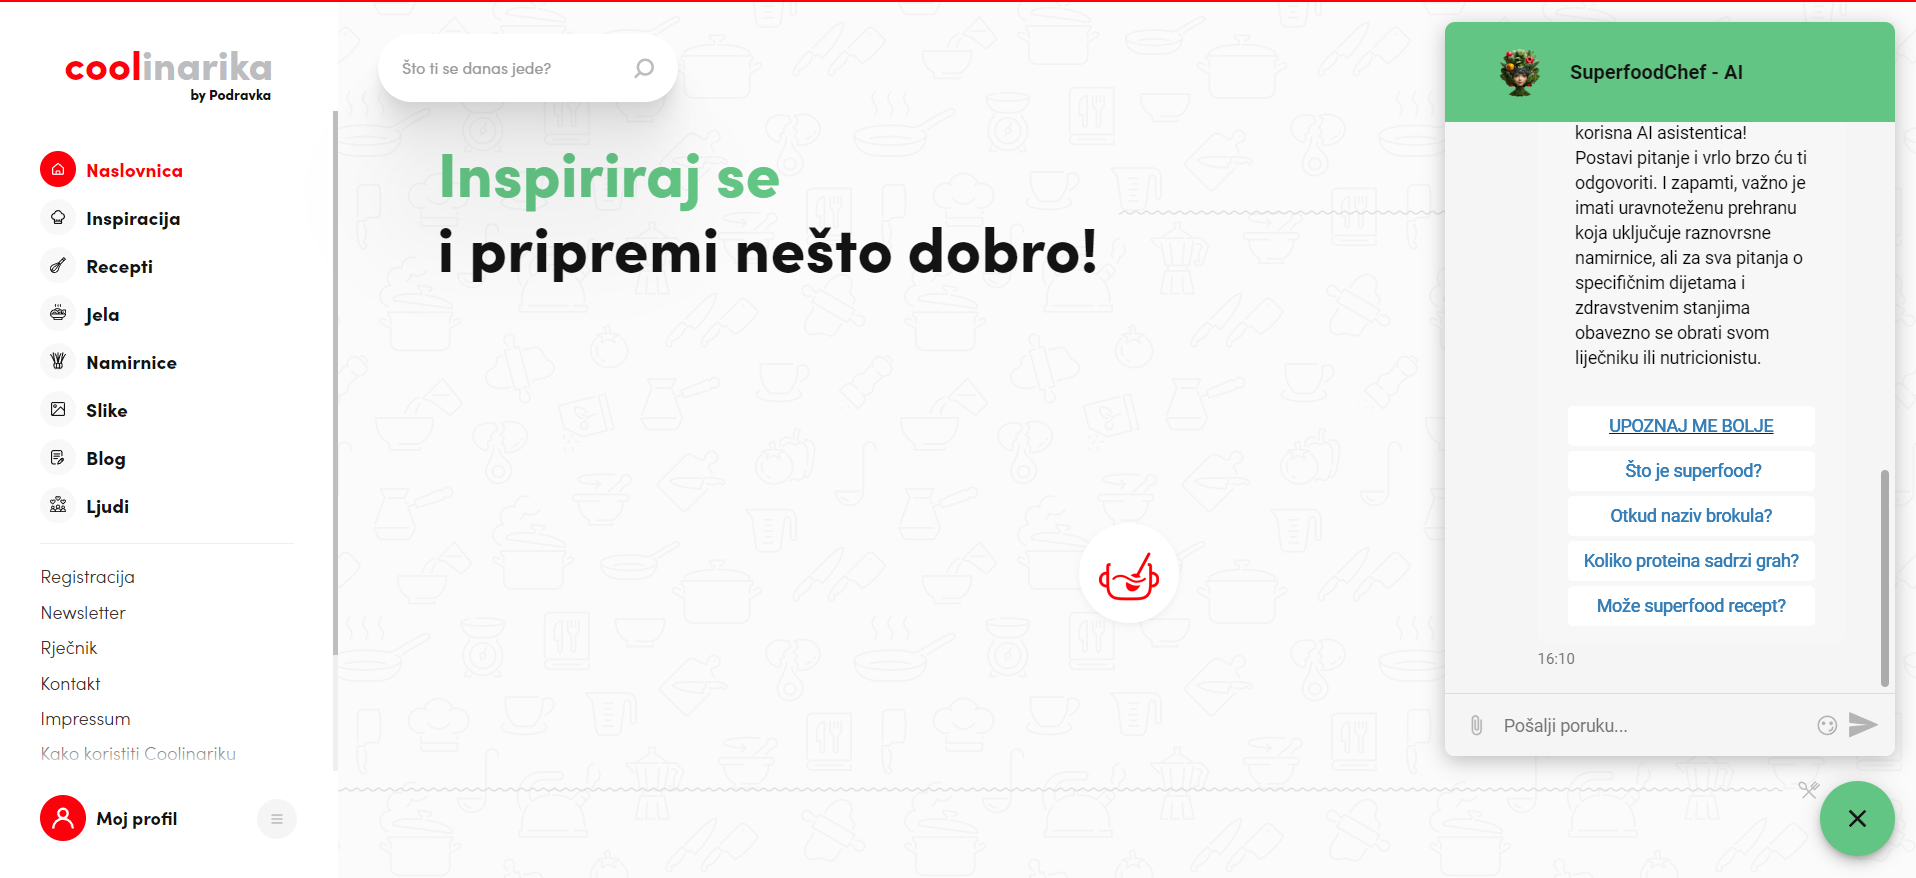
\includegraphics[scale= 0.3]{slike/coolinarka.png}
			\centering
			\caption{Coolinarka}
			\label{fig:Coolinarka}
		\end{figure} 
		
		\begin{figure}[H]
			
\includegraphics[scale= 0.3]{slike/recipeci.png}
			\centering
			\caption{ReciPeci}
			\label{fig:ReciPeci}
		\end{figure} 
		
		
		\noindent U prijašnjem odlomku spomenuli smo prednost odlične kategorizacije ove aplikacije pa tako gdje se ta prednost pokazuje jest upravo tako što imamo kategorije hrane za mlade, kategorije hrane za osobe sa bolestima te za starije osobe kojima odgovara lagana prehrana.\\
		
		\noindent Tako naša aplikacija zahvaća razne kategorije ljudi kao što su:
		\begin{packed_item}
			\item \textit{mlađe osobe koje tek uče kuhati}
			\item \textit{osobe koje ne stignu raditi duge pripreme}
			\item \textit{starije osobe koje ne mogu pripremati i konzumirati svu hranu}
			\item \textit{odrasli koji žele naučiti kuhati}
			\item \textit{osobe koje žele izraditi kompliciranije stvari sa nešto manje kulinarskog iskustva}
		\end{packed_item}
		
		\noindent Sama aplikacija od razvoja pa do konačne aplikacije i poslije je vrlo lako prilagodljiva. Osim izvornih alata pisanja koda, dijelove aplikacije lako je prilagoditi u smislu izgleda, dodavanja novih kategorija, dodatnih opcija privatnog profila. Ako želimo znati zašto, to je jednostavno. Cijela aplikacija u kodu je strukturirana na način da se prate i učitavaju određene strukture sa podatcima gdje je tada u slučaju bilo kakve modifikacije potrebno promjenu učiniti na samo jednom mjestu.\\
		
		\noindent Što se samih promjena tiče, aplikacija se sastoji od više verzija. Kod razvoja aplikacije u pogon se pušta prvo prototip koji sadrži osnovnu funkcionalnost zbog potrebe provjere ispravnosti aplikacije. U sljedećim verzijama aplikacija se nadograđuje profilima korisnika, poslovnim i privatnim profilima pa se nadalje dodaje i kategorije, izbornici, i slično te u konačnici mogućnost komunikacije između autora i recenzije njihovih recepata. \\
		
		\noindent Nakon završetka postavljenih ciljeva pri izradi aplikacije, zbog same strukture i čitljivosti pri pisanju, aplikaciju je u naknadnim verzijama moguće nadograditi sa brojnim drugim značajkama.\\
		Primjer takvih značajki:
		
		\begin{packed_item}
			\item \textit{komunikacija unutar aplikacije putem videopoziva}
			\item \textit{AI pomoć pri odabiru recepta i kategorije}
			\item \textit{AI stvaranje jelovnika prilagođenog za dan i posebne prilike}
			\item \textit{Stvaranje odjela za događaje izrade i objave novih recepata}
			\item \textit{Tečajevi za kuhanje putem videa i videopoziva}
		\end{packed_item}
		
	
		
		
		
		\eject
		
	
	\chapter{Specifikacija programske potpore}
		
	\section{Funkcionalni zahtjevi}
			
			\textbf{\textit{dio 1. revizije}}\\
			
			\textit{Navesti \textbf{dionike} koji imaju \textbf{interes u ovom sustavu} ili  \textbf{su nositelji odgovornosti}. To su prije svega korisnici, ali i administratori sustava, naručitelji, razvojni tim.}\\
				
			\textit{Navesti \textbf{aktore} koji izravno \textbf{koriste} ili \textbf{komuniciraju sa sustavom}. Oni mogu imati inicijatorsku ulogu, tj. započinju određene procese u sustavu ili samo sudioničku ulogu, tj. obavljaju određeni posao. Za svakog aktora navesti funkcionalne zahtjeve koji se na njega odnose.}\\
			
			
			\noindent \textbf{Dionici:}
			
			\begin{packed_enum}
				
				\item Dionik 1
				\item Dionik 2				
				\item ...
				
			\end{packed_enum}
			
			\noindent \textbf{Aktori i njihovi funkcionalni zahtjevi:}
			
			
			\begin{packed_enum}
				\item  \underbar{Aktor 1 (inicijator) može:}
				
				\begin{packed_enum}
					
					\item funkcionalnost 1
					\item funkcionalnost 2
					\begin{packed_enum}
						
						\item  podfunkcionalnost 1 
						\item  podfunkcionalnost 2
				
					\end{packed_enum}
					\item  funkcionalnost 3
					
				\end{packed_enum}
			
				\item  \underbar{Aktor 2 (sudionik) može:}
				
				\begin{packed_enum}
					
					\item funkcionalnost 1
					\item funkcionalnost 2
					
				\end{packed_enum}
			\end{packed_enum}
			
			\eject 
			
			
				
			\subsection{Obrasci uporabe}
				
				
						\noindent \underbar{\textbf{UC1 - Pregled recepata}}
					\begin{packed_item}
						
						\item \textbf{Glavni sudionik: Neregistiran korisnik, Registriran korisnik}
						\item  \textbf{Cilj: Pregled recepata temeljem kategorija} 
						\item  \textbf{Sudionici: Baza podataka} 
						\item  \textbf{Preduvjet: -} 
						\item  \textbf{Opis osnovnog tijeka:}
						
						\item[] \begin{packed_enum}
							
							\item Korisnik otvori platformu
							\item Ponuđene su mu kategorije, vrste kuhinje, specifični sastojci
							\item Korisnik odabire kategoriju i prikazuju mu se recepti
						\end{packed_enum}
						
						\item  \textbf{Opis mogućih odstupanja:}
						
						\item[] \begin{packed_item}
							
							\item[2.a] 
							\item[] \begin{packed_enum}
								
								\item 
								\item
								
							\end{packed_enum}
							\item[2.b] 
							\item[3.a] 
							
						\end{packed_item}
					\end{packed_item}
					
					
					\noindent \underbar{\textbf{UC2 - Registracija}}
					\begin{packed_item}
						
						\item \textbf{Glavni sudionik: Neregistrirani korisnik}
						\item  \textbf{Cilj: Stvaranje računa za pristup ostalim značajkama sustava}  
						\item  \textbf{Sudionici: Baza podtaka} 
						\item  \textbf{Preduvjet:-} 
						\item  \textbf{Opis osnovnog tijeka:}
						
						\item[] \begin{packed_enum}
							
							\item Korisnik odabire opciju za registraciju
							\item Korisnik unosi potrebne korisničke podatke
							\item Korisnik prima obavijest o uspješnoj registraciji
						\end{packed_enum}
						
						\item  \textbf{Opis mogućih odstupanja:}
						
						\item[] \begin{packed_item}
							
							\item[2.a] Odabir već zauzetog korisničkog imena i/ili e-maila, unos korisničkog podatka u nedozvoljenom formatu ili pružanje neispravnoga e-maila
							\item[] \begin{packed_enum}
								
								\item  Sustav obavještava korisnika o neuspjelom upisu i vraća ga na stranicu za registraciju
								\item Korisnik mijenja potrebne podatke te završava unos ili odustaje od registracije
								
							\end{packed_enum}
							
						\end{packed_item}
					\end{packed_item}
					
					
					\noindent \underbar{\textbf{UC3 - Prijava u sustav}}
					\begin{packed_item}
						
						\item \textbf{Glavni sudionik: }
						\item  \textbf{Cilj:} 
						\item  \textbf{Sudionici:} 
						\item  \textbf{Preduvjet:} 
						\item  \textbf{Opis osnovnog tijeka:}
						
						\item[] \begin{packed_enum}
							
							\item 
							\item 
							\item 
							\item 
							\item 
						\end{packed_enum}
						
						\item  \textbf{Opis mogućih odstupanja:}
						
						\item[] \begin{packed_item}
							
							\item[2.a] 
							\item[] \begin{packed_enum}
								
								\item 
								\item
								
							\end{packed_enum}
							\item[2.b] 
							\item[3.a] 
							
						\end{packed_item}
					\end{packed_item}
					
					\noindent \underbar{\textbf{UC4 - Objava recepata}}
					\begin{packed_item}
						
						\item \textbf{Glavni sudionik: Registrirani korisnik }
						\item  \textbf{Cilj: Objava svog recepta na stranici} 
						\item  \textbf{Sudionici:} 
						\item  \textbf{Preduvjet: Registracija i prijava korisnika} 
						\item  \textbf{Opis osnovnog tijeka:}
						
						\item[] \begin{packed_enum}
							
							\item 
							\item 
							\item 
							\item 
							\item 
						\end{packed_enum}
						
						\item  \textbf{Opis mogućih odstupanja:}
						
						\item[] \begin{packed_item}
							
							\item[2.a] 
							\item[] \begin{packed_enum}
								
								\item 
								\item
								
							\end{packed_enum}
							\item[2.b] 
							\item[3.a] 
							
						\end{packed_item}
					\end{packed_item}
					
					\noindent \underbar{\textbf{UC5 - Razmjena poruka}}
					\begin{packed_item}
						
						\item \textbf{Glavni sudionik: }
						\item  \textbf{Cilj:} 
						\item  \textbf{Sudionici:} 
						\item  \textbf{Preduvjet:} 
						\item  \textbf{Opis osnovnog tijeka:}
						
						\item[] \begin{packed_enum}
							
							\item 
							\item 
							\item 
							\item 
							\item 
						\end{packed_enum}
						
						\item  \textbf{Opis mogućih odstupanja:}
						
						\item[] \begin{packed_item}
							
							\item[2.a] 
							\item[] \begin{packed_enum}
								
								\item 
								\item
								
							\end{packed_enum}
							\item[2.b] 
							\item[3.a] 
							
						\end{packed_item}
					\end{packed_item}
					
					\noindent \underbar{\textbf{UC6 - Čavrljanje }}
					\begin{packed_item}
						
						\item \textbf{Glavni sudionik: }
						\item  \textbf{Cilj:} 
						\item  \textbf{Sudionici:} 
						\item  \textbf{Preduvjet:} 
						\item  \textbf{Opis osnovnog tijeka:}
						
						\item[] \begin{packed_enum}
							
							\item 
							\item 
							\item 
							\item 
							\item 
						\end{packed_enum}
						
						\item  \textbf{Opis mogućih odstupanja:}
						
						\item[] \begin{packed_item}
							
							\item[2.a] 
							\item[] \begin{packed_enum}
								
								\item 
								\item
								
							\end{packed_enum}
							\item[2.b] 
							\item[3.a] 
							
						\end{packed_item}
					\end{packed_item}
					
					\noindent \underbar{\textbf{UC7 - Videopoziv}}
					\begin{packed_item}
						
						\item \textbf{Glavni sudionik: }
						\item  \textbf{Cilj:} 
						\item  \textbf{Sudionici:} 
						\item  \textbf{Preduvjet:} 
						\item  \textbf{Opis osnovnog tijeka:}
						
						\item[] \begin{packed_enum}
							
							\item 
							\item 
							\item 
							\item 
							\item 
						\end{packed_enum}
						
						\item  \textbf{Opis mogućih odstupanja:}
						
						\item[] \begin{packed_item}
							
							\item[2.a] 
							\item[] \begin{packed_enum}
								
								\item 
								\item
								
							\end{packed_enum}
							\item[2.b] 
							\item[3.a] 
							
						\end{packed_item}
					\end{packed_item}
					
					
				\subsubsection{Dijagrami obrazaca uporabe}
					
					\textit{Prikazati odnos aktora i obrazaca uporabe odgovarajućim UML dijagramom. Nije nužno nacrtati sve na jednom dijagramu. Modelirati po razinama apstrakcije i skupovima srodnih funkcionalnosti.}
				\eject		
				
			\subsection{Sekvencijski dijagrami}
				
				\noindent
				\textbf{Obrazac uporabe UC1-Pregled recepata}\newline
					{Korisnik šalje zahtjev za prikaz recepata po kategorijama, sastojcima i/ili kuhinjama kojim pripadaju. Poslužitelj dohvaća recepete koji zadovoljavaju uvjete i prikazuje ih korisniku. Korisnik sada može spremiti recepte, ako je prijavljen to se provodi, ako nije preusmjeri ga se na stranicu za prijavu.}
				
				
				\begin{figure}[H]
					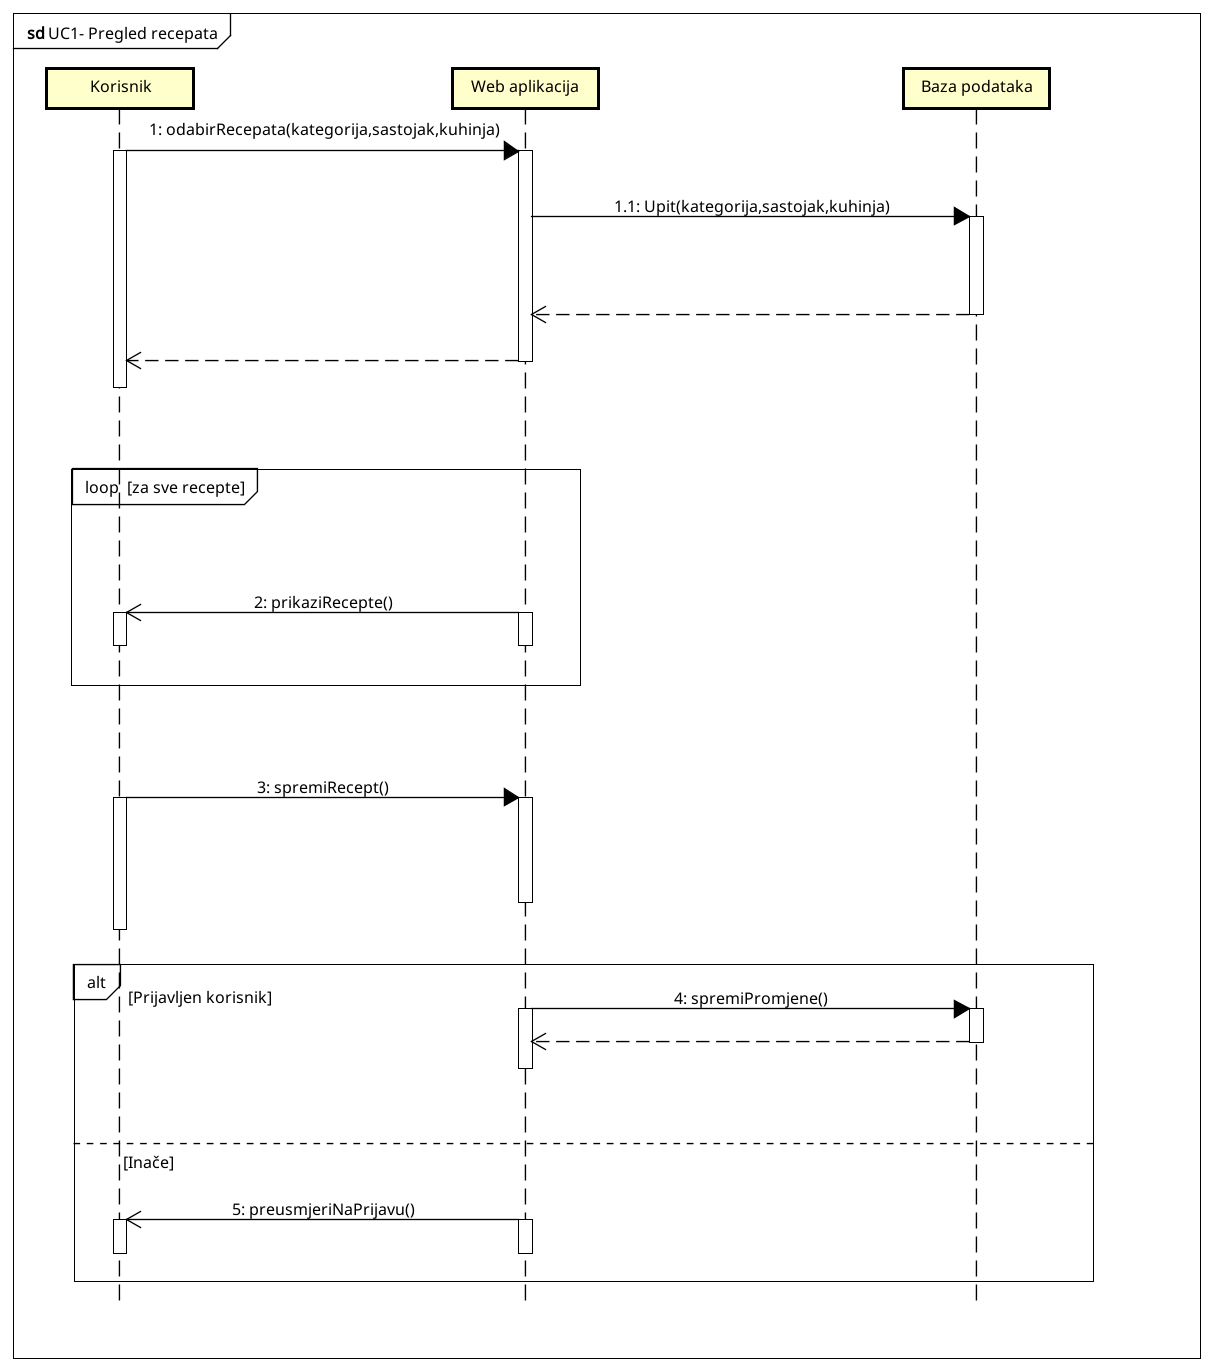
\includegraphics[scale= 0.4]{slike/sekvencijski_dijagramUC1.png}
					\centering
					\caption{Sekvencijski dijagram za UC1}
					\label{fig:Sekvencijski dijagram za UC1}
				\end{figure} 
				\eject

				\noindent
				\textbf{Obrazac uporabe UC3-Registracija}\newline
					{Korisnik se registrira s korisničkim imenom i lozinkom. Ako takav korisnik već postoji, korisniku se ispisuje greška. Inače, korisnik se uspješno registrirao i to se bilježi u bazi podataka.}
				

				\begin{figure}[H]
					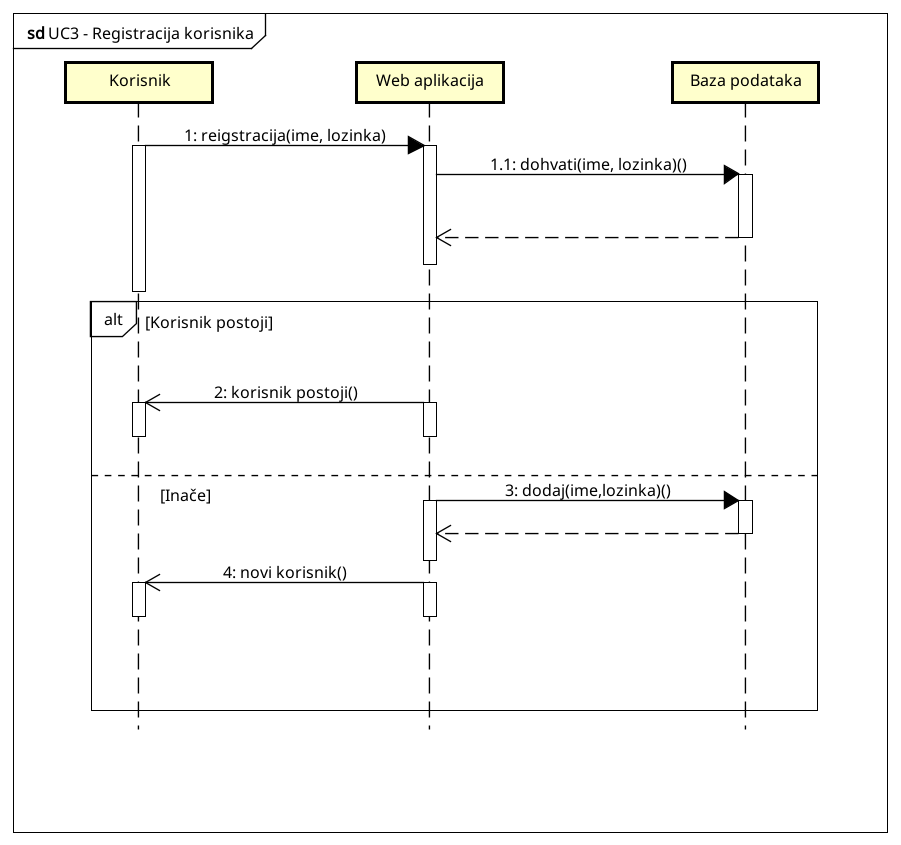
\includegraphics[scale= 0.6]{slike/sekvencijski_dijagramUC3.png}
					\centering
					\caption{Sekvencijski dijagram za UC3}
					\label{fig:Sekvencijski dijagram za UC3}
				\end{figure}
				
				\eject

				\noindent
				\textbf{Obrazac uporabe UC4-Prijava Korisnika}\newline
					{Korisnik pokuša objaviti novi recept. Ako nije prijavljen, preusmjeri ga se na prijavu. Inače, recept se dodaje u bazu podataka i o tome se obavijesti korisnik.}
				

				\begin{figure}[H]
					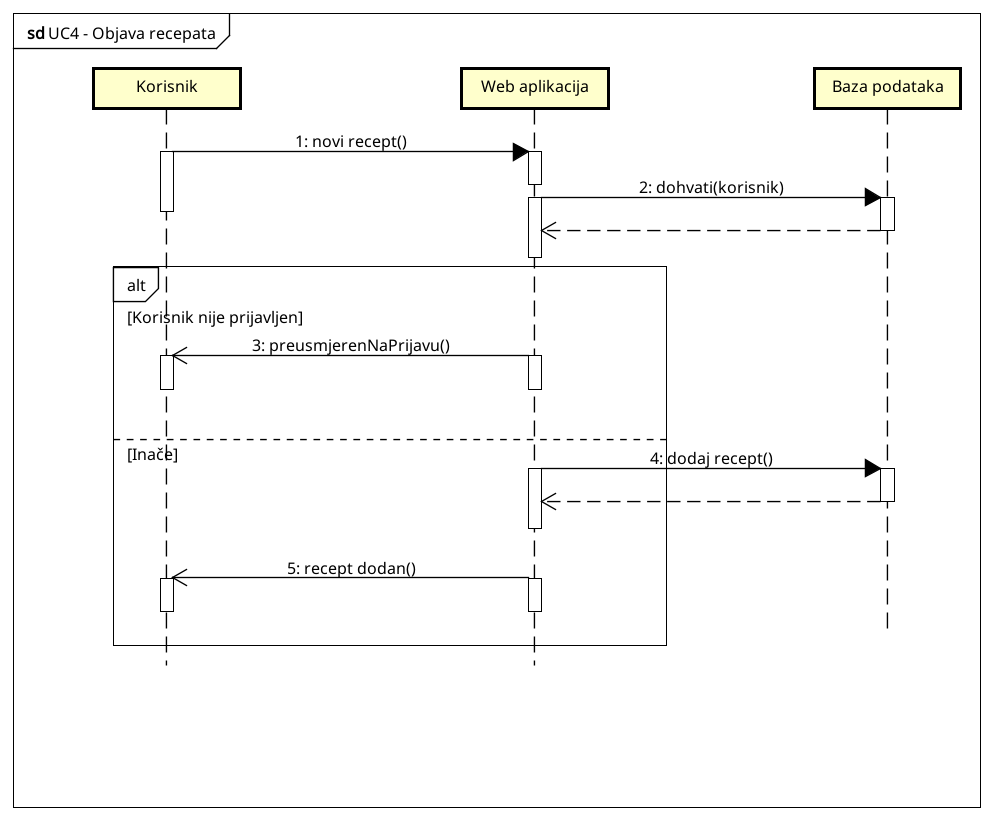
\includegraphics[scale= 0.6]{slike/sekvencijski_dijagramUC4.png}
					\centering
					\caption{Sekvencijski dijagram za UC4}
					\label{fig:Sekvencijski dijagram za UC4}
				\end{figure}

				\eject

				\noindent
				\textbf{Obrazac uporabe UC8-Videopoziv}\newline
					{Korisnik zatraži video poziv s drugim korisnikom. Ako drugi korisnik ne postoji, poziv se ne uspostavlja i o tome se obavijesti prvog korisnika. Inače se šalje zahtjev za video pozivom drugom korisniku, koji ga može odbiti ili prihvatiti. Ako odbije poziv se ne uspostavlja i o tome se obavijesti prvi korsnik. Ako prihvati uspostavi se video poziv između dva korisnika.}
				

				\begin{figure}[H]
					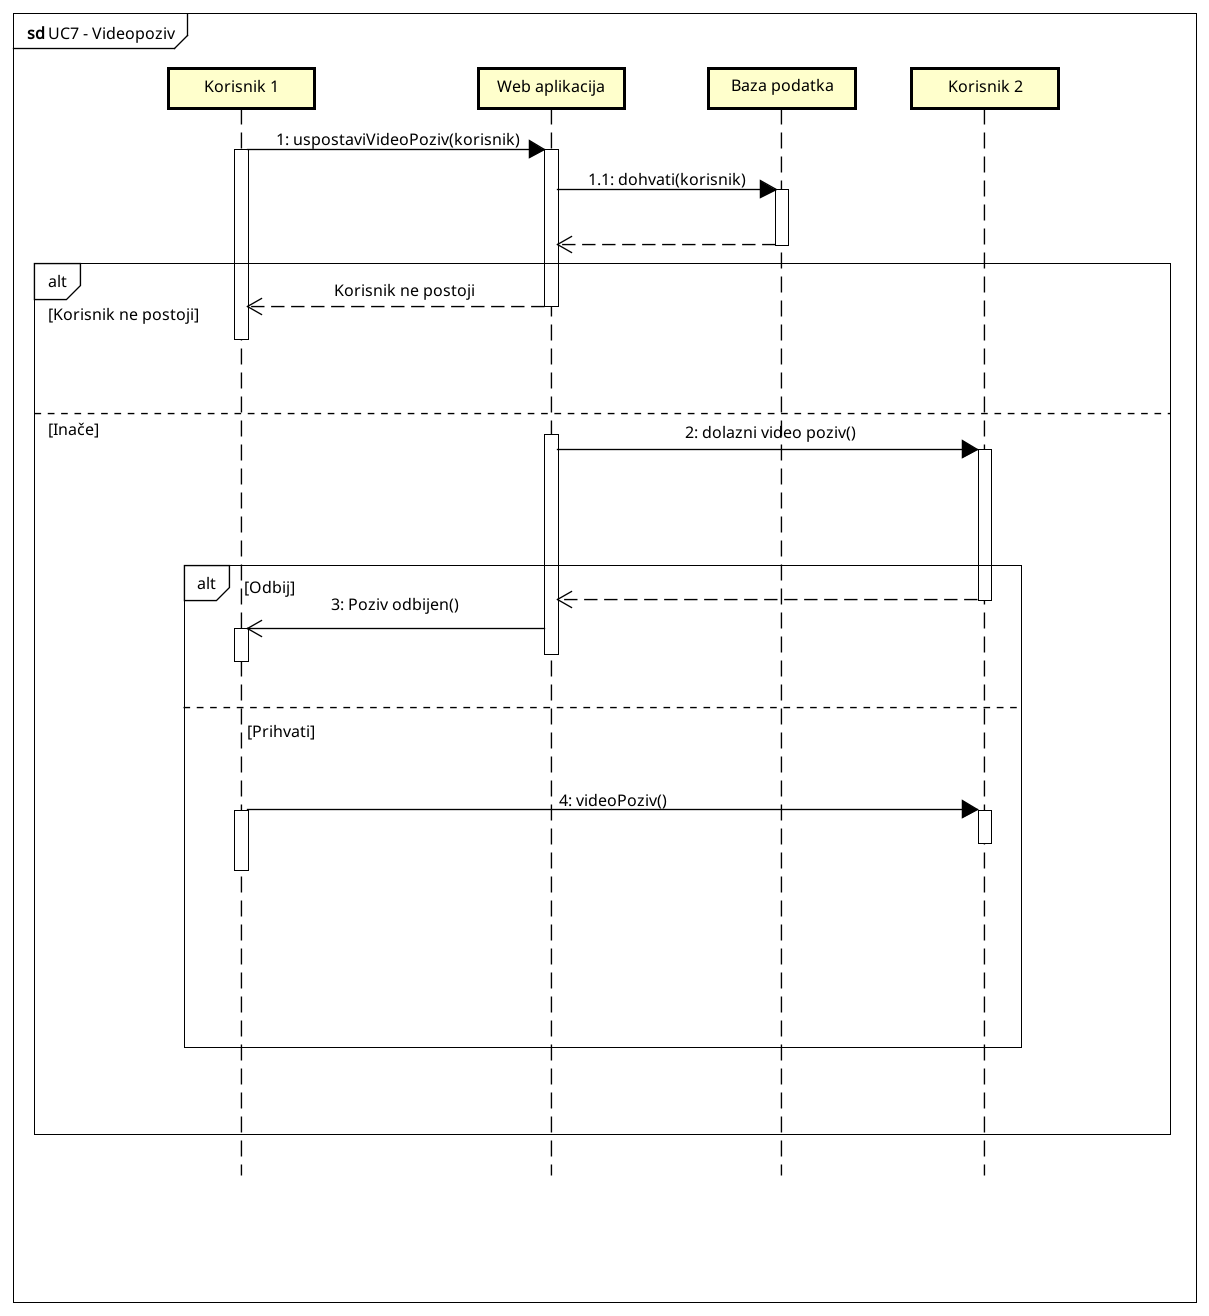
\includegraphics[scale= 0.5]{slike/sekvencijski_dijagramUC7.png}
					\centering
					\caption{Sekvencijski dijagram za UC7}
					\label{fig:Sekvencijski dijagram za UC7}
				\end{figure}
				
				\eject
			
			\section{Ostali zahtjevi}
		
			\textit{Nefunkcionalne zahtjeve koji će se navesti u nastavku teksta pojašnjavaju dodatne zahtjeve koje web aplikacija treba koristiti ili već koristi.}
			
			\begin{packed_item}
				
				\item Sustav treba biti implementiran kao web aplikacija koristeći objektno-orijentirane paradigme i norme kako bi se omogućilo ponovno korištenje dijelova koda/modula.
				\item Nepravilno korištenje web aplikacije ne smije rezultirati padom sustava, odnosno potrebno je usmjeriti korisnika na pravilno korištenje informacionim obavještenjima.
				\item U sustavu treba biti omogućen rad i korištenje web aplikacije od strane više korisnika (cca. 50).
				\item Sustav treba omogućiti komuniciranje korisnika s ostalim korisnicima putem tekstualnog chat-a i video poziva.
				\item Sustav mora podržati dijakritičke znakove hrvatskoj jezika, dakle treba podržati hrvatsku abecedu. Omogućit će se i promjena jezika s hrvatskog na engleski jezik.
				\item Hrvatski jezik je zadani jezik unutar web aplikacije.
				\item Sustav mora imati intuitivno sučelje koje neće stvarati nedoumice kod korisnika odnosno web-aplikacija treba biti jednostavna za korištenje.
				\item Konekcija s bazom podataka mora imati brz odziv. Bilo kakav pokušaj neovlaštenog pristupa informacijama u bazi podataka potrebno je spriječiti i istu adekvatno zašititi.
				\item Web aplikacija koristi proces kripitiranja lozinki za prijavu korisnika koji se tako u hash-ovima spremaju u bazu podataka.
				\item Sustav mora omogućiti korištenje određenih funkcionalnosti samo prijavljenim/registriranim korisnicima.
				\item Učitavanje početne stranice web aplikacije ne smije trajati duže od 5 sekundi.
				\item Pristup sustavu i razmjena podataka se vrši HTTPS protokolom.
				\item Pri razvoju web aplikacije koristi se React Native i Spring framework u Java programskom jeziku.
				
			\end{packed_item}
			 
			 
			 
	
	\chapter{Arhitektura i dizajn sustava}

\textnormal{Arhitektura sustava je bazirana na tri komponente koje komuniciraju jedna s drugom. Odnosno, sustav je podijeljen u tri dolje navedena sloja, a koji se mogu prikazati slikom ispod.}
\begin{itemize}
	\item 	\textit{Web poslužitelj}
	\item 	\textit{Web aplikacija}
	\item 	\textit{Baza podataka}
\end{itemize}

\begin{figure}[H]
	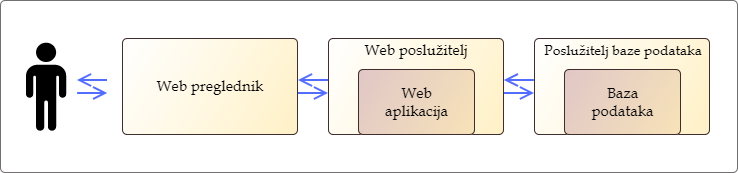
\includegraphics[width=\textwidth]{slike/arhitekturaSustava.png} %veličina slike u odnosu na originalnu datoteku i pozicija slike
	\centering
	\caption{Arhitektura sustava}
	\label{fig:arhitekturasustava}
\end{figure}

\textnormal{\textbf{Web preglednik} omogućava korisniku prikaz web stranice koja pruža određene funkcionalnosti. Omogućava prikaz web stranice (prikaz videa, slika i ostalog multimedijalnog sadržaja) onako kako je definirana u datotekama, dakle omogućuje interpretiranje koda u koristan oblik "običnom" korisniku.
	Putem web preglednika korisnik šalje zahtjev za željenu radnju koja se onda proslijedi idućim koponentama na obradu, te nakon obrade opet se prikazuju u vidljivom obliku kao vid povratne informacije.}

\textnormal{\textbf{Web poslužitelj} je ključna komponenta u obradi korisničkih zahtjeva.
	Dakle, to je \textbf{središnji dio} aplikacije koji omogućava komunikaciju korisnika s aplikacijom.
	U središnjem sloju se odvijaju procesi koji su zaslužni za komunikaciju s bazom podataka ukoliko je to potrebno, a to se odvija
	prema MVC (Model - View - Controller) arhitekturnom obrascu. Model definira podatkovnu strukturu entiteta baze podataka,
	View (pogled) upravlja izgledom i prikazom sadržaja korisniku u web pregledniku, te Controller (kontroler) upravlja i reagira
	na korisničke događaje.
	Odnos komponenti predstavljen je slikom \ref{fig:arhitekturasustava2}.}

\begin{figure}[H]
	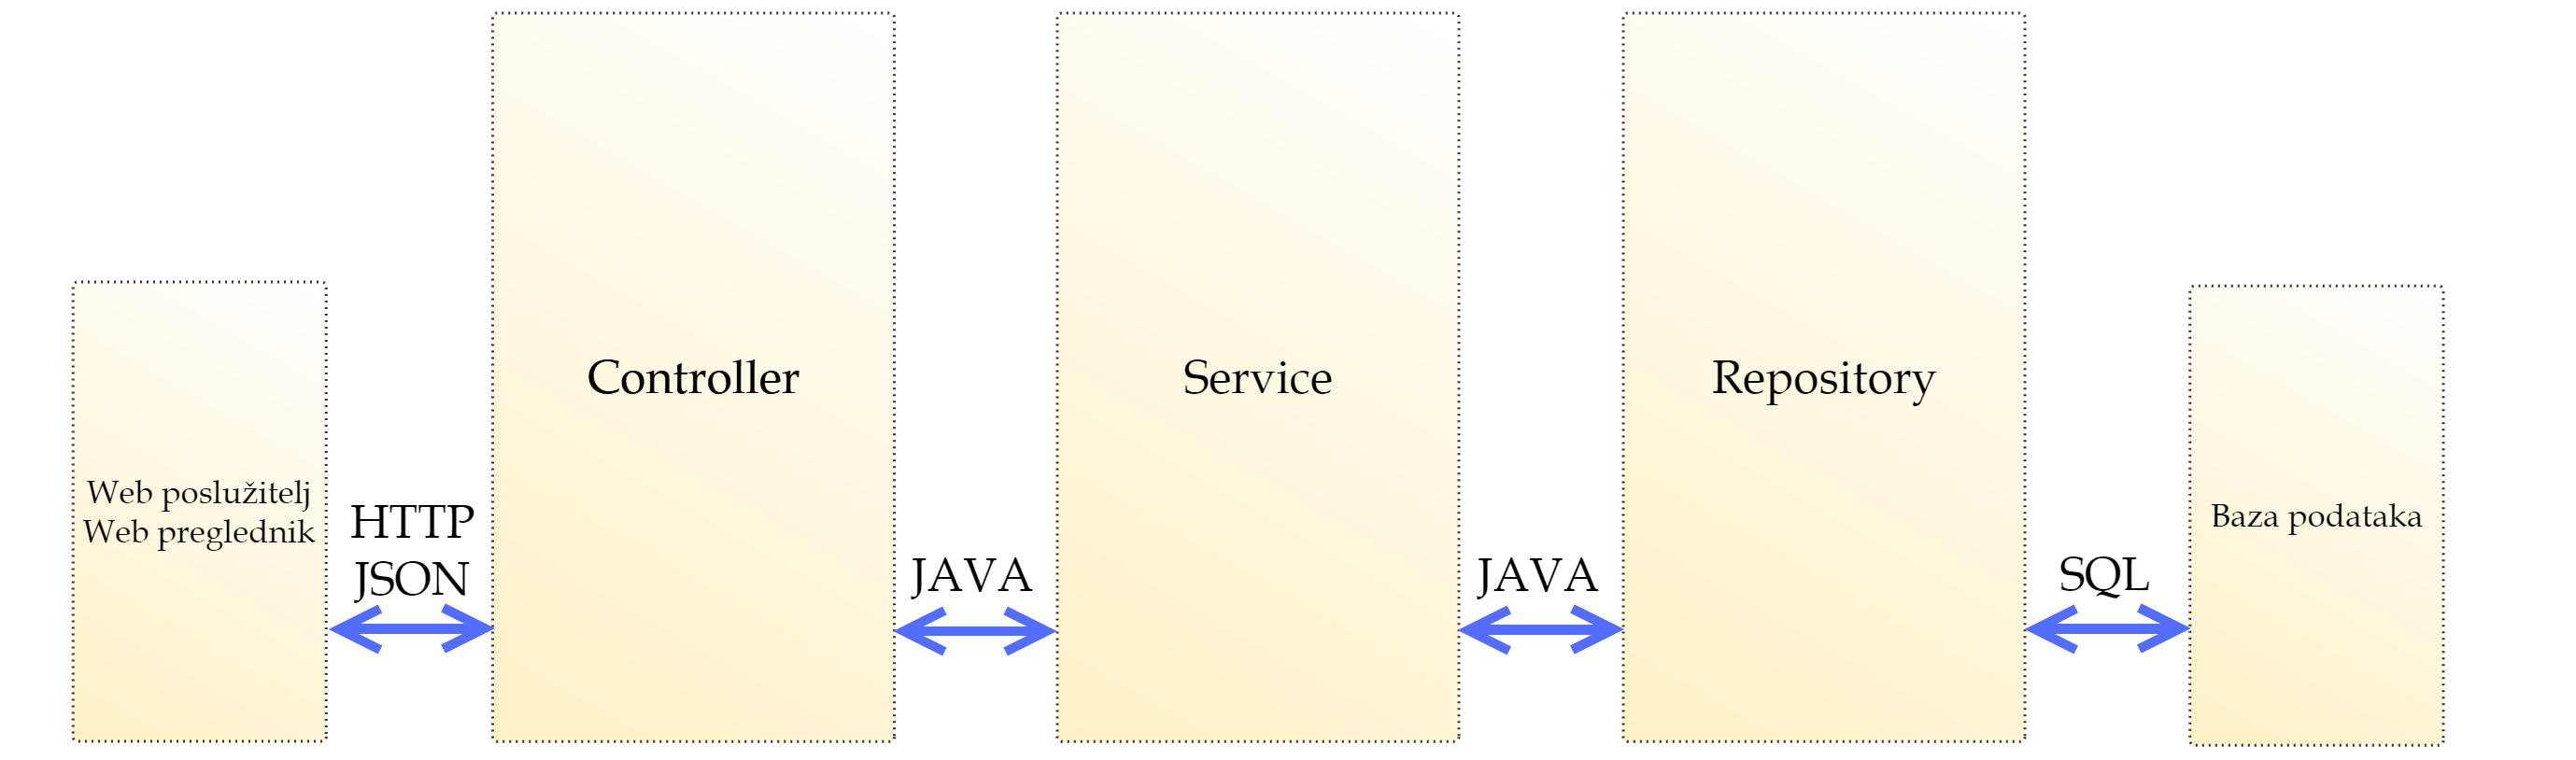
\includegraphics[width=\textwidth]{slike/arhitekturaSustava2.png} %veličina slike u odnosu na originalnu datoteku i pozicija slike
	\centering
	\caption{Arhitektura sustava backend}
	\label{fig:arhitekturasustava2}
\end{figure}

\textnormal{Za izradu ovakve web aplikacije kako bi se pokrile navedene specifične funkcionalnosti koristit će se Spring framework za Javu, te React za prikaz na web pregledniku u radnom okruženju IntelliJIDEA.
	Specifično za Spring framework, koristit će se navedeni tip arhitekture kao što je naveden slikom \ref{fig:arhitekturasustava2}, jer će se putem metoda JPARepository moći upravljati zahtjevima korisnika koji se vežu za upite u bazi podataka.
	Ukratko, obavljaju se operacije nad \textbf{PostgreSQL bazom podataka}.}

\textnormal{\textbf{Kontroler} upravlja korisničkim zahtjevima i prosljeđuje ih dalje prema \textbf{Service} gdje se obavlja logika nad upitima i zahtjevima. Service komunicira s \textbf{bazom podataka} preko JPARepository.}

\textnormal{UI će biti povezan sa ostalim dijelovima web aplikacije putem \textbf{REST servisa}, odnosno REST servis preko HTTP zahtjeva omogućuje pristup funkcijama za upravljanje bazom podataka. Nad bazom podataka se mogu vršiti  (CRUD - Create, Read, Update, Delete) operacije. Takva vrsta komunikacije je predstavljena slikom \ref{fig:arhitekturasustava3}.
	UI je izveden uz pomoć \textbf{React} framework-a koji se koristi komponentama za organizaciju prikaza.}

\begin{figure}[H]
	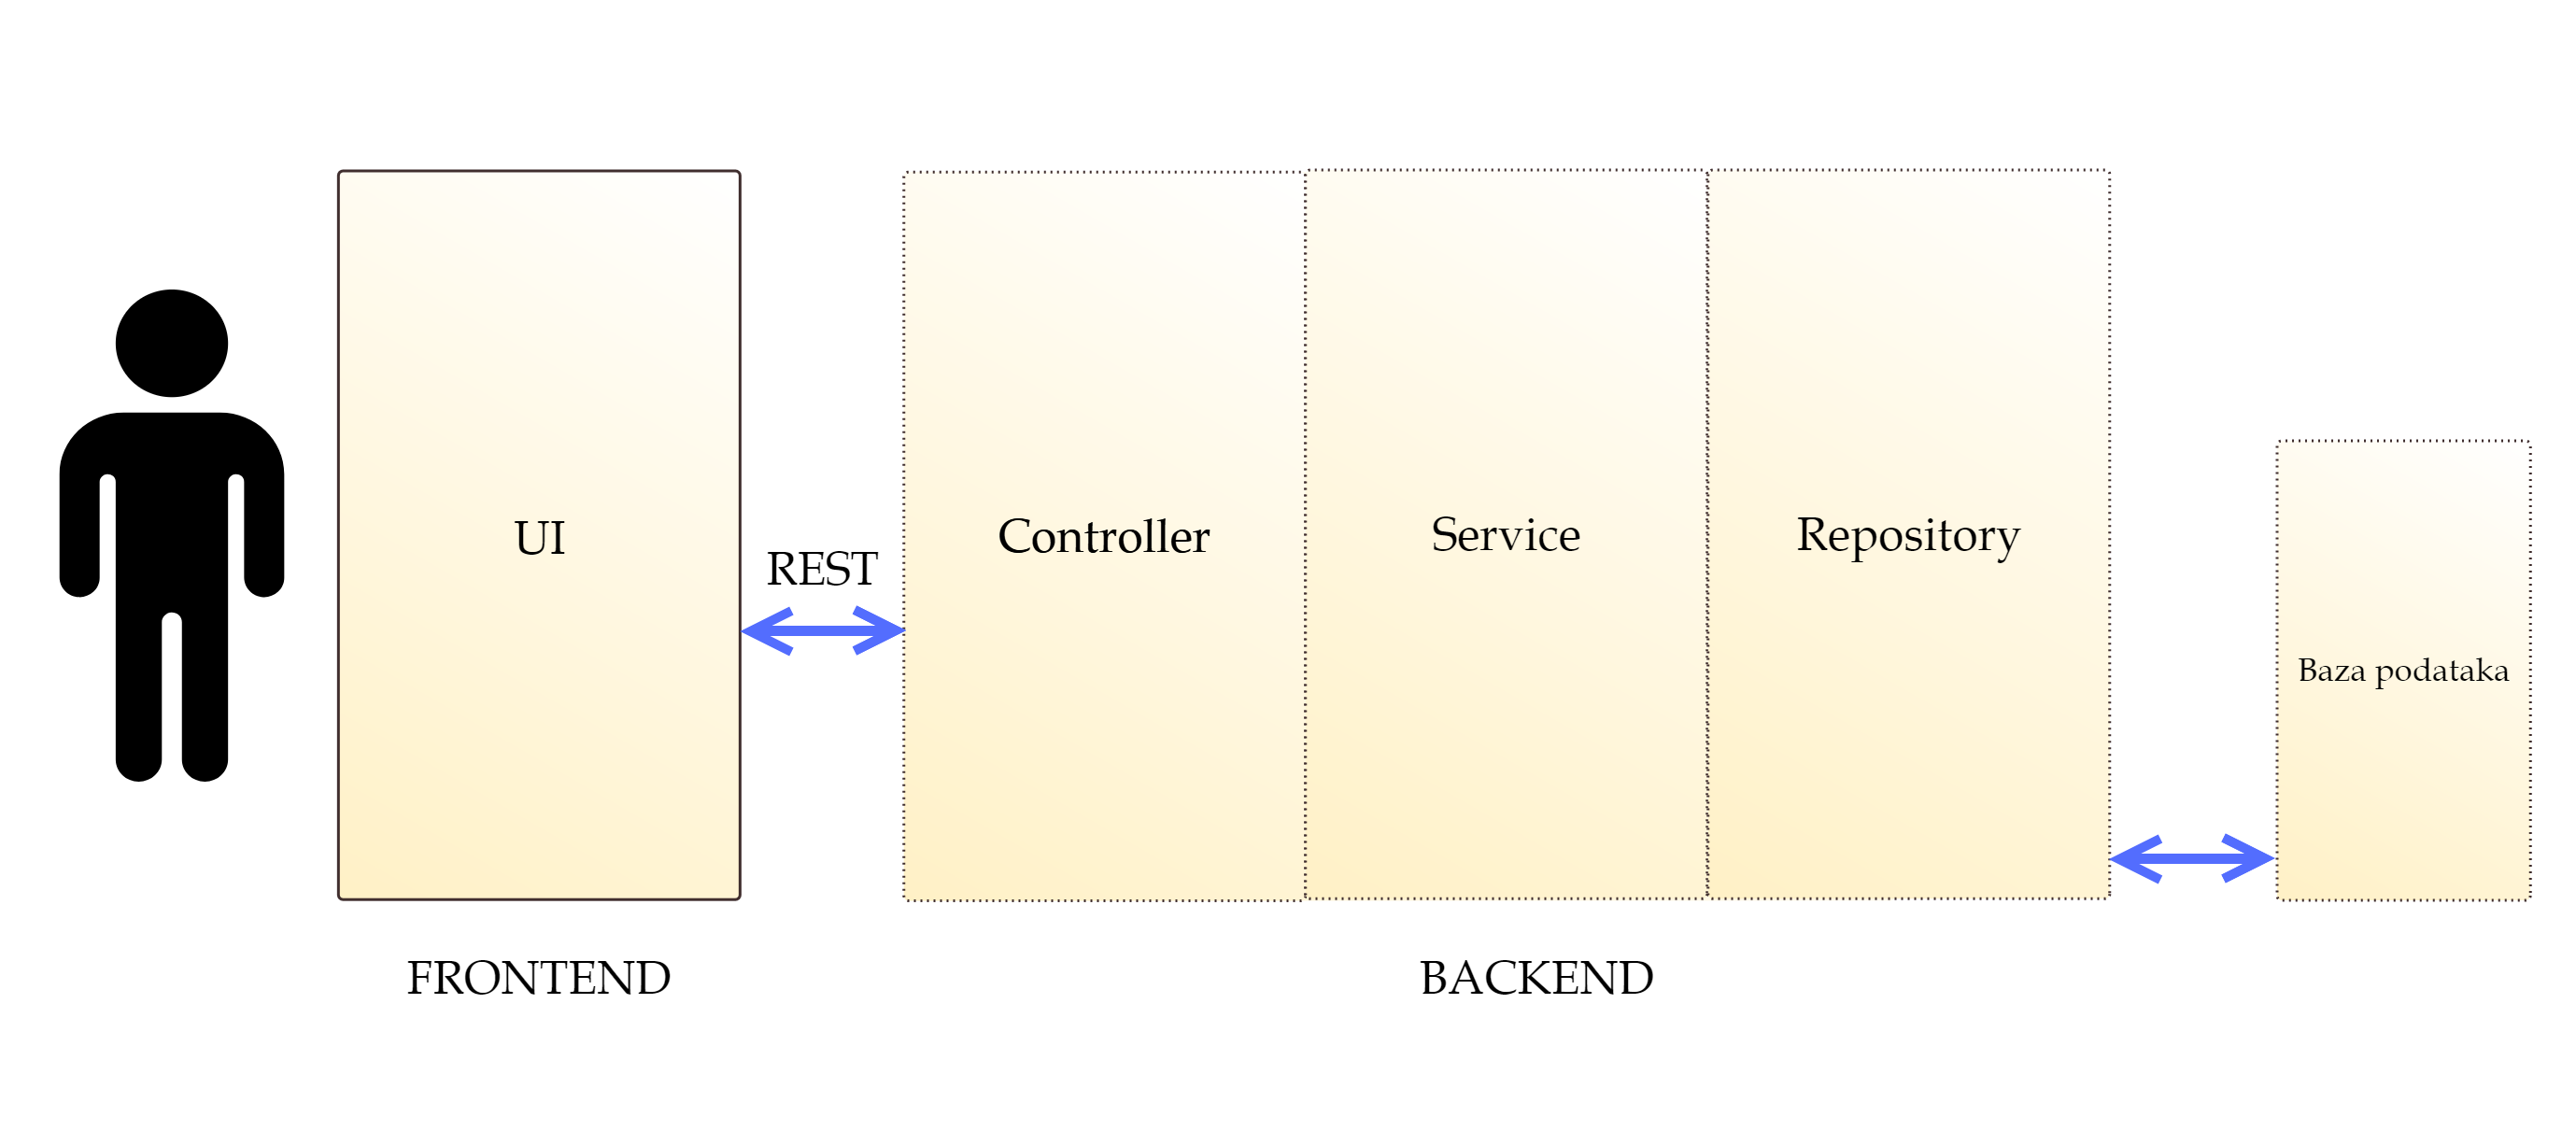
\includegraphics[width=\textwidth]{slike/arhitekturaSustava3.png} %veličina slike u odnosu na originalnu datoteku i pozicija slike
	\centering
	\caption{Arhitektura sustava backend i frontend}
	\label{fig:arhitekturasustava3}
\end{figure}

\eject





\section{Baza podataka}


\textnormal{Kao rješenje za web aplikaciju koju izrađujemo, odlučili smo se na relacijski model baze podataka jer nam ona omogućava precizno oblikovanje i modeliranje elemenata iz stvarnog svijeta. Međusobni odnos tablica se zasniva na relaciji dok se svaka tablica sastoji od naziva entiteta te njegovih pripadajućih atributa koji opisuju dani entitet. Ovakav tip baze podataka u ovom slučaju nam omogućava brzo spremanje, dohvat i izmjenu (uređivanje ili brisanje) podataka koji cirkulišu u web aplikaciji. Baza podataka koja je spremna za izradu ove web aplikacije se sastoji od sljedećih elemenata/tablica:}

\begin{packed_item}

	\item Korisnik
	\item Recept
	\item Kategorija
	\item ReceptKategorije
	\item ReceptSastojci
	\item Sastojak
	\item KomentariRecept
	\item Komentar
	\item Pratioci
	\item OznačavanjeRecepata
	\item SpremljenRecept
	\item VrsteKuhinjeRecepata
	\item VrstaKuhinja
	\item Obavijesti

\end{packed_item}

\eject

\subsection{Opis tablica}


\textnormal{\textbf{Korisnik}		Entitet Korisnik služi za evidenciju podataka o korisnicima koji koriste web aplikaciju. Atributi koji ga opisuju su korisnickoIme, lozinkaKorisnik, imeKorisnik, prezimeKorisnik, brojTelefona, emailKorisnik, razinaOvlasti i Dostupan što označava kada je dostupan za komunikaciju s drugim korisnicima unutar web aplikacije. Entitet Korisnik je u \textit{One-To-Many} vezi s entitetom Recept. Entitet Korisnik je i u \textit{Many-To-Many} vezi s entitetom OmiljeniAutor koji bilježi korisnike koje ovaj korisnik prati. Također, ovaj entitet je u \textit{Many-To-Many} vezi s entitetima SpremljenRecept, OznačenRecept, a u \textit{One-To-Many} vezi s entitetima Objava i Komentar.}


\begin{longtblr}[
	label=none,
	entry=none
	]{
	width = \textwidth,
	colspec={|X[8,l]|X[6, l]|X[20, l]|},
	rowhead = 1,
	} %definicija širine tablice, širine stupaca, poravnanje i broja redaka naslova tablice
	\hline \SetCell[c=3]{c}{\textbf{Korisnik}}                                     \\ \hline[3pt]
	\SetCell{LightGreen}IDKorisnik & INT     & jedinstveni identifikator korisnika \\ \hline
	KorisnickoIme                  & VARCHAR & korisničko ime                      \\ \hline
	LozinkaKorisnik                & VARCHAR & spremljena hash lozinka za pristup  \\ \hline
	ImeKorisnik                    & VARCHAR & ime korisnika                       \\ \hline
	PrezimeKorisnik                & VARCHAR & prezime korisnika                   \\ \hline
	BrojTelefona                   & VARCHAR & broj telefona korisnika             \\ \hline
	EmailKorisnik                  & VARCHAR & e-mail adresa korisnika             \\ \hline
	RazinaOvlasti                  & VARCHAR & razina ovlasti u aplikaciji         \\ \hline
	DostupanOd                     & TIME    & vrijeme dostupnosti                 \\ \hline
	DostupanDo                     & TIME    & vrijeme dostupnosti                 \\ \hline
\end{longtblr}

\eject

\textnormal{\textbf{Komentar}		Entitet Komentar služi za evidenciju komentara koji korisnici međusobno dijele u web aplikaciji. Opisuju ga atributi IDKomentar, IDKorisnik, SadrzajKomentar i DatumKomentar. Ovaj entitet je  u \textit{Many-To-One} vezi s entitetom Korisnik.}

\begin{longtblr}[
	label=none,
	entry=none
	]{
	width = \textwidth,
	colspec={|X[8,l]|X[6, l]|X[20, l]|},
	rowhead = 1,
	} %definicija širine tablice, širine stupaca, poravnanje i broja redaka naslova tablice
	\hline \SetCell[c=3]{c}{\textbf{Komentar}}                                     \\ \hline[3pt]
	\SetCell{LightGreen}IDKomentar & INT     & jedinstveni identifikator komentara \\ \hline
	\SetCell{LightBlue}IDKorisnik  & INT     & jedinstveni identifikator korisnika \\ \hline
	OpisKomentar                   & VARCHAR & sadržaj komentara                   \\ \hline
	DatumKomentar                  & DATE    & datum komentara                     \\ \hline
\end{longtblr}

\textnormal{\textbf{KomentariRecept}		Entitet KomentariRecept služi za evidenciju komentara. Ovaj entitet je  u \textit{Many-To-Many} vezi s entitetom Korisnik.}

\begin{longtblr}[
	label=none,
	entry=none
	]{
	width = \textwidth,
	colspec={|X[8,l]|X[6, l]|X[20, l]|},
	rowhead = 1,
	} %definicija širine tablice, širine stupaca, poravnanje i broja redaka naslova tablice
	\hline \SetCell[c=3]{c}{\textbf{KomentariRecept}}                          \\ \hline[3pt]
	\SetCell{LightGreen}ID         & INT & jedinstveni identifikator           \\ \hline
	\SetCell{LightGreen}IDKomentar & INT & jedinstveni identifikator komentara \\ \hline
	\SetCell{LightBlue}IDRecept    & INT & jedinstveni identifikator recepta   \\ \hline
\end{longtblr}


\vspace{\baselineskip}
\textnormal{\textbf{Pratioci}		Entitet Pratioci služi za evidenciju korisnika koje jedan korisnik zaprati. Opisan je sljedećim atributima: IDKorisnik i IDAutor. U \textit{Many-To-Many} je vezi s entitetom Korisnik unutar web aplikacije.}

\begin{longtblr}[
	label=none,
	entry=none
	]{
	width = \textwidth,
	colspec={|X[6,l]|X[6, l]|X[20, l]|},
	rowhead = 1,
	} %definicija širine tablice, širine stupaca, poravnanje i broja redaka naslova tablice
	\hline \SetCell[c=3]{c}{\textbf{Pratioci}}                                 \\ \hline[3pt]
	\SetCell{LightGreen}ID        & INT & jedinstveni identifikator            \\ \hline
	\SetCell{LightBlue}IDKorisnik & INT & jedinstveni identifikator pratitelja \\ \hline
	\SetCell{LightBlue}IDAutor    & INT & ID korisnika koji je zapraćen        \\ \hline
\end{longtblr}

\vspace{\baselineskip}
\textnormal{\textbf{Recept}		Entitet Recept služi za evidenciju podataka o receptima koji cirkulišu i nastaju u web aplikaciji. Opisan je atributima: IDRecept, NazivRecept, IDKategorija, IDSastojak, IDVrstaKuhinja, PripremaRecept, VrijemeKuhanja, IDOznaka, SlikaRecept i IDVideoRecept. Entitet Recept je u \textit{Many-To-One} vezi s entitetom Korisnik, a u \textit{Many-To-Many} vezi s entitetom Sastojak, te u \textit{Many-To-Many} vezi s Kategorija, a \textit{One-To-One} s VrstaKuhinja. Također je u \textit{One-To-One} vezi s entitetom Objava.}

\begin{longtblr}[
	label=none,
	entry=none
	]{
	width = \textwidth,
	colspec={|X[8,l]|X[6, l]|X[20, l]|},
	rowhead = 1,
	} %definicija širine tablice, širine stupaca, poravnanje i broja redaka naslova tablice
	\hline \SetCell[c=3]{c}{\textbf{Recept}}                                           \\ \hline[3pt]
	\SetCell{LightGreen}IDRecept      & INT     & jedinstveni identifikator recepta    \\ \hline
	NazivRecept                       & VARCHAR & naziv recepta                        \\ \hline
	\SetCell{LightBlue}IDKategorija   & INT     & ID kategorije kojoj recept pripada   \\ \hline
	\SetCell{LightBlue}IDSastojak     & INT     & ID sastojka u receptu                \\ \hline
	\SetCell{LightBlue}IDVrstaKuhinja & INT     & ID vrste kuhinje recepta             \\ \hline
	PripremaRecept                    & VARCHAR & Opis pripreme recepta                \\ \hline
	VrijemeKuhanja                    & TIME    & Vrijeme potrebno za pripremu recepta \\ \hline
	Oznaka                            & INT     & Oznaka recepta                       \\ \hline
	SlikaRecept                       & VARCHAR & Slika recepta                        \\ \hline
	VideoRecept                       & VARCHAR & Video recepta                        \\ \hline
\end{longtblr}

\vspace{\baselineskip}
\textnormal{\textbf{OznačavanjeRecepata}		Entitet OznačavanjeRecepata služi za evidenciju označenih recepata od strane korisnika. Opisan je atributima: IDRecept i IDKorisnik. U \textit{Many-To-Many} vezi je s entitetom Korisnik.}

\begin{longtblr}[
	label=none,
	entry=none
	]{
	width = \textwidth,
	colspec={|X[6,l]|X[6, l]|X[20, l]|},
	rowhead = 1,
	} %definicija širine tablice, širine stupaca, poravnanje i broja redaka naslova tablice
	\hline \SetCell[c=3]{c}{\textbf{OznačavanjeRecepata}}                     \\ \hline[3pt]
	\SetCell{LightGreen}ID        & INT & jedinstveni identifikator           \\ \hline
	\SetCell{LightBlue}IDRecept   & INT & jedinstveni identifikator recepta   \\ \hline
	\SetCell{LightBlue}IDKorisnik & INT & ID korisnika koji je označio recept \\ \hline
\end{longtblr}

\vspace{\baselineskip}
\textnormal{\textbf{SpremljenRecept}		Entitet SpremljenRecept za evidenciju spremljenih recepata od strane korisnika. Opisan je atributima: IDRecept i IDKorisnik. U \textit{Many-To-Many} vezi je s entitetom Korisnik.}

\begin{longtblr}[
	label=none,
	entry=none
	]{
	width = \textwidth,
	colspec={|X[6,l]|X[6, l]|X[20, l]|},
	rowhead = 1,
	} %definicija širine tablice, širine stupaca, poravnanje i broja redaka naslova tablice
	\hline \SetCell[c=3]{c}{\textbf{SpremljenRecept}}                         \\ \hline[3pt]
	\SetCell{LightGreen}ID        & INT & jedinstveni identifikator           \\ \hline
	\SetCell{LightBlue}IDRecept   & INT & jedinstveni identifikator recepta   \\ \hline
	\SetCell{LightBlue}IDKorisnik & INT & ID korisnika koji je spremio recept \\ \hline
\end{longtblr}

\vspace{\baselineskip}
\textnormal{\textbf{Kategorija}		Entitet Kategorija služi za evidenciju kategorija. Opisan je atributima: IDKategorija, NazivKategorija.}

\begin{longtblr}[
	label=none,
	entry=none
	]{
	width = \textwidth,
	colspec={|X[8,l]|X[6, l]|X[20, l]|},
	rowhead = 1,
	} %definicija širine tablice, širine stupaca, poravnanje i broja redaka naslova tablice
	\hline \SetCell[c=3]{c}{\textbf{Kategorija}}                                      \\ \hline[3pt]
	\SetCell{LightGreen}IDKategorija & INT     & jedinstveni identifikator kateogrije \\ \hline
	NazivKategorija                  & VARCHAR & naziv kategorije                     \\ \hline
\end{longtblr}

\vspace{\baselineskip}
\textnormal{\textbf{ReceptKategorije}		Entitet ReceptKategorije služi za evidenciju kategorija i recepata pod tim kategorijama. Opisan je atributima: IDKategorija, NazivKategorija. U \textit{Many-To-Many} vezi je s entitetom Recept.}

\begin{longtblr}[
	label=none,
	entry=none
	]{
	width = \textwidth,
	colspec={|X[8,l]|X[6, l]|X[20, l]|},
	rowhead = 1,
	} %definicija širine tablice, širine stupaca, poravnanje i broja redaka naslova tablice
	\hline \SetCell[c=3]{c}{\textbf{ReceptKategorije}}                           \\ \hline[3pt]
	\SetCell{LightGreen}ID          & INT & jedinstveni identifikator            \\ \hline
	\SetCell{LightBlue}IDRecept     & INT & jedinstveni identifikator kateogrije \\ \hline
	\SetCell{LightBlue}IDKategorija & INT & jedinstveni identifikator recepta    \\ \hline
\end{longtblr}

\vspace{\baselineskip}
\textnormal{\textbf{VrstaKuhinja}		Entitet VrstaKuhinja služi za evidenciju različitih vrsta kuhinja. Opisan je atributima: IDVrstaKuhinja, NazivVrstaKuhinja. U \textit{One-To-One} vezi je s entitetom Recept.}

\begin{longtblr}[
	label=none,
	entry=none
	]{
	width = \textwidth,
	colspec={|X[9,l]|X[6, l]|X[20, l]|},
	rowhead = 1,
	} %definicija širine tablice, širine stupaca, poravnanje i broja redaka naslova tablice
	\hline \SetCell[c=3]{c}{\textbf{VrstaKuhinja}}                                         \\ \hline[3pt]
	\SetCell{LightGreen}IDVrstaKuhinje & INT     & jedinstveni identifikator vrste kuhinje \\ \hline
	NazivVrstaKuhinja                  & VARCHAR & naziv vrste kuhinje                     \\ \hline
\end{longtblr}

\vspace{\baselineskip}
\textnormal{\textbf{VrsteKuhinjeRecepata}		Entitet VrsteKuhinjeRecepata služi za evidenciju različitih vrsta kuhinja recepta ukoliko je to prikladno za recept (nije određeno kojoj pripada).}

\begin{longtblr}[
	label=none,
	entry=none
	]{
	width = \textwidth,
	colspec={|X[9,l]|X[6, l]|X[20, l]|},
	rowhead = 1,
	} %definicija širine tablice, širine stupaca, poravnanje i broja redaka naslova tablice
	\hline \SetCell[c=3]{c}{\textbf{VrsteKuhinjeRecepata}}                                    \\ \hline[3pt]
	\SetCell{LightGreen}ID            & INT & jedinstveni identifikator               \\ \hline
	\SetCell{LightBlue}IDVrstaKuhinje & INT & jedinstveni identifikator vrste kuhinje \\ \hline
	\SetCell{LightBlue}IDRecept       & INT & jedinstveni identifikator recepta       \\ \hline
\end{longtblr}

\vspace{\baselineskip}
\textnormal{\textbf{Sastojak}		Entitet Sastojak služi za evidenciju različitih sastojaka. Opisan je atributima: IDSastojak, NazivSastojak.}

\begin{longtblr}[
	label=none,
	entry=none
	]{
	width = \textwidth,
	colspec={|X[6,l]|X[6, l]|X[20, l]|},
	rowhead = 1,
	} %definicija širine tablice, širine stupaca, poravnanje i broja redaka naslova tablice
	\hline \SetCell[c=3]{c}{\textbf{Sastojak}}                                    \\ \hline[3pt]
	\SetCell{LightGreen}IDSastojak & INT     & jedinstveni identifikator sastojka \\ \hline
	NazivSastojak                  & VARCHAR & naziv sastojka                     \\ \hline
\end{longtblr}

\vspace{\baselineskip}
\textnormal{\textbf{ReceptSastojci}		Entitet ReceptSastojci služi za evidenciju različitih sastojaka unutar recepta. Opisan je atributima: IDRecept, IDSastojak. U \textit{Many-To-Many} vezi je s entitetom Recept.}

\begin{longtblr}[
	label=none,
	entry=none
	]{
	width = \textwidth,
	colspec={|X[8,l]|X[6, l]|X[20, l]|},
	rowhead = 1,
	} %definicija širine tablice, širine stupaca, poravnanje i broja redaka naslova tablice
	\hline \SetCell[c=3]{c}{\textbf{ReceptSastojci}}                         \\ \hline[3pt]
	\SetCell{LightGreen}ID        & INT & jedinstveni identifikator          \\ \hline
	\SetCell{LightBlue}IDRecept   & INT & jedinstveni identifikator recepta  \\ \hline
	\SetCell{LightBlue}IDSastojak & INT & jedinstveni identifikator sastojka \\ \hline
\end{longtblr}

\vspace{\baselineskip}
\textnormal{\textbf{Obavijesti}		Entitet Obavijesti služi za slanje obavijesti korisnicima koji prate određene autore recepata. Opisan je atributima: IDObavijest, IDAutor, NazivObavijest, SadrzajObavijest, DatumObavijest i JeProcitano. U \textit{Many-To-One} vezi je s entitetom Korisnik.}

\begin{longtblr}[
	label=none,
	entry=none
	]{
	width = \textwidth,
	colspec={|X[8,l]|X[6, l]|X[20, l]|},
	rowhead = 1,
	} %definicija širine tablice, širine stupaca, poravnanje i broja redaka naslova tablice
	\hline \SetCell[c=3]{c}{\textbf{Obavijesti}}                                    \\ \hline[3pt]
	\SetCell{LightGreen}IDObavijest & INT     & jed. identifikator obavijesti       \\ \hline
	\SetCell{LightBlue}IDKorisnik   & INT     & jedinstveni identifikator korisnika \\ \hline
	NazivObavijest                  & VARCHAR & naziv obavijesti                    \\ \hline
	SadrzajObavijest                & VARCHAR & sadržaj obavijesti                  \\ \hline
	DatumObavijest                  & DATE    & datum obavijesti                    \\ \hline
	JeProcitano                     & TINYINT & oznaka pročitane obavijesti         \\ \hline
\end{longtblr}

\subsection{Dijagram baze podataka}
%unos slike
\begin{figure}[H]
	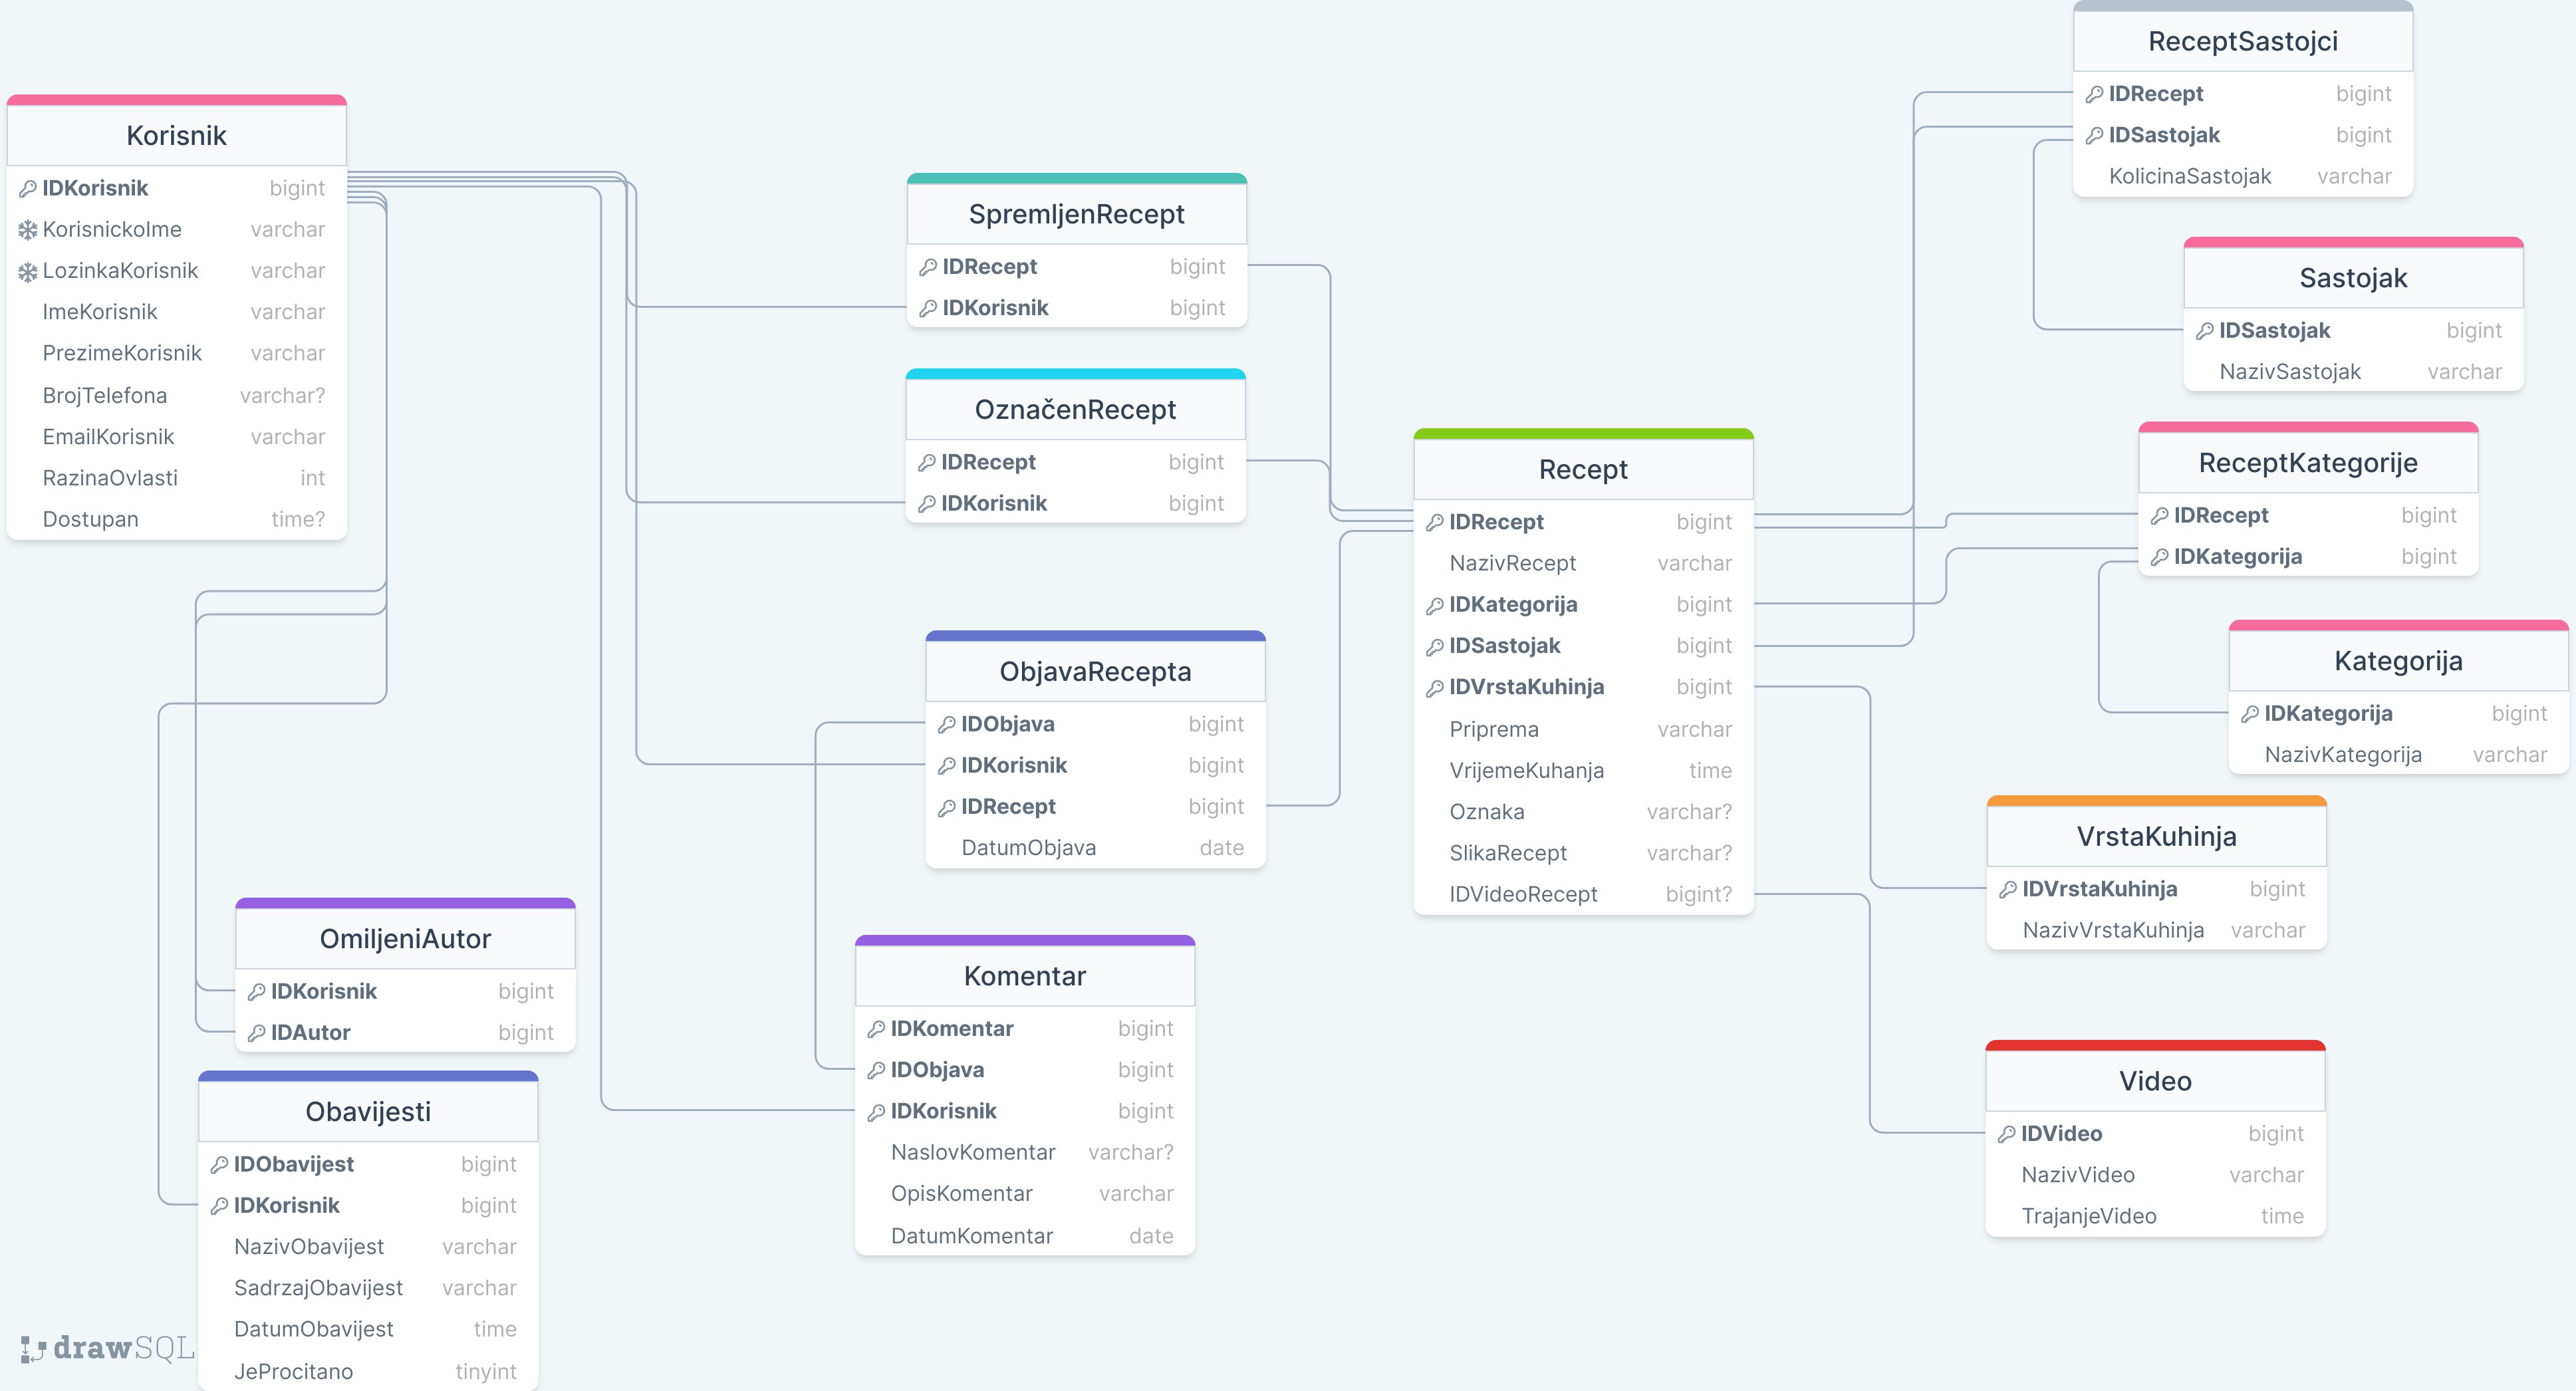
\includegraphics[width=\textwidth]{slike/CookBooked-dbp.png} %veličina slike u odnosu na originalnu datoteku i pozicija slike
	\centering
	\caption{Dijagram relacijske baze podataka za web aplikaciju}
	\label{fig:dijagrambp}
\end{figure}
\eject


\section{Dijagram razreda}

\textit{Potrebno je priložiti dijagram razreda s pripadajućim opisom. Zbog preglednosti je moguće dijagram razlomiti na više njih, ali moraju biti grupirani prema sličnim razinama apstrakcije i srodnim funkcionalnostima.}\\

\textbf{\textit{dio 1. revizije}}\\

\textit{Prilikom prve predaje projekta, potrebno je priložiti potpuno razrađen dijagram razreda vezan uz \textbf{generičku funkcionalnost} sustava. Ostale funkcionalnosti trebaju biti idejno razrađene u dijagramu sa sljedećim komponentama: nazivi razreda, nazivi metoda i vrste pristupa metodama (npr. javni, zaštićeni), nazivi atributa razreda, veze i odnosi između razreda.}\\

\textbf{\textit{dio 2. revizije}}\\

\textit{Prilikom druge predaje projekta dijagram razreda i opisi moraju odgovarati stvarnom stanju implementacije}



\eject

\section{Dijagram stanja}


\textbf{\textit{dio 2. revizije}}\\

\textit{Potrebno je priložiti dijagram stanja i opisati ga. Dovoljan je jedan dijagram stanja koji prikazuje \textbf{značajan dio funkcionalnosti} sustava. Na primjer, stanja korisničkog sučelja i tijek korištenja neke ključne funkcionalnosti jesu značajan dio sustava, a registracija i prijava nisu. }


\eject

\section{Dijagram aktivnosti}

\textbf{\textit{dio 2. revizije}}\\

\textit{Potrebno je priložiti dijagram aktivnosti s pripadajućim opisom. Dijagram aktivnosti treba prikazivati značajan dio sustava.}

\eject
\section{Dijagram komponenti}

\textbf{\textit{dio 2. revizije}}\\

\textit{Potrebno je priložiti dijagram komponenti s pripadajućim opisom. Dijagram komponenti treba prikazivati strukturu cijele aplikacije.}
	\chapter{Implementacija i korisničko sučelje}
		
		
		\section{Korištene tehnologije i alati}
		
			\textbf{\textit{dio 2. revizije}}
			
			 \textit{Detaljno navesti sve tehnologije i alate koji su primijenjeni pri izradi dokumentacije i aplikacije. Ukratko ih opisati, te navesti njihovo značenje i mjesto primjene. Za svaki navedeni alat i tehnologiju je potrebno \textbf{navesti internet poveznicu} gdje se mogu preuzeti ili više saznati o njima}.
			
			
			\eject 
		
	
		\section{Ispitivanje programskog rješenja}
			
			\textbf{\textit{dio 2. revizije}}\\
			
			 \textit{U ovom poglavlju je potrebno opisati provedbu ispitivanja implementiranih funkcionalnosti na razini komponenti i na razini cijelog sustava s prikazom odabranih ispitnih slučajeva. Studenti trebaju ispitati temeljnu funkcionalnost i rubne uvjete.}
	
			
			\subsection{Ispitivanje komponenti}
			\textit{Potrebno je provesti ispitivanje jedinica (engl. unit testing) nad razredima koji implementiraju temeljne funkcionalnosti. Razraditi \textbf{minimalno 6 ispitnih slučajeva} u kojima će se ispitati redovni slučajevi, rubni uvjeti te izazivanje pogreške (engl. exception throwing). Poželjno je stvoriti i ispitni slučaj koji koristi funkcionalnosti koje nisu implementirane. Potrebno je priložiti izvorni kôd svih ispitnih slučajeva te prikaz rezultata izvođenja ispita u razvojnom okruženju (prolaz/pad ispita). }
			
			
			
			\subsection{Ispitivanje sustava}
			
			 \textit{Potrebno je provesti i opisati ispitivanje sustava koristeći radni okvir Selenium\footnote{\url{https://www.seleniumhq.org/}}. Razraditi \textbf{minimalno 4 ispitna slučaja} u kojima će se ispitati redovni slučajevi, rubni uvjeti te poziv funkcionalnosti koja nije implementirana/izaziva pogrešku kako bi se vidjelo na koji način sustav reagira kada nešto nije u potpunosti ostvareno. Ispitni slučaj se treba sastojati od ulaza (npr. korisničko ime i lozinka), očekivanog izlaza ili rezultata, koraka ispitivanja i dobivenog izlaza ili rezultata.\\ }
			 
			 \textit{Izradu ispitnih slučajeva pomoću radnog okvira Selenium moguće je provesti pomoću jednog od sljedeća dva alata:}
			 \begin{itemize}
			 	\item \textit{dodatak za preglednik \textbf{Selenium IDE} - snimanje korisnikovih akcija radi automatskog ponavljanja ispita	}
			 	\item \textit{\textbf{Selenium WebDriver} - podrška za pisanje ispita u jezicima Java, C\#, PHP koristeći posebno programsko sučelje.}
			 \end{itemize}
		 	\textit{Detalji o korištenju alata Selenium bit će prikazani na posebnom predavanju tijekom semestra.}
			
			\eject 
		
		
		\section{Dijagram razmještaja}
			
			\textbf{\textit{dio 2. revizije}}
			
			 \textit{Potrebno je umetnuti \textbf{specifikacijski} dijagram razmještaja i opisati ga. Moguće je umjesto specifikacijskog dijagrama razmještaja umetnuti dijagram razmještaja instanci, pod uvjetom da taj dijagram bolje opisuje neki važniji dio sustava.}
			
			\eject 
		
		\section{Upute za puštanje u pogon}
		
			\textbf{\textit{dio 2. revizije}}\\
		
			 \textit{U ovom poglavlju potrebno je dati upute za puštanje u pogon (engl. deployment) ostvarene aplikacije. Na primjer, za web aplikacije, opisati postupak kojim se od izvornog kôda dolazi do potpuno postavljene baze podataka i poslužitelja koji odgovara na upite korisnika. Za mobilnu aplikaciju, postupak kojim se aplikacija izgradi, te postavi na neku od trgovina. Za stolnu (engl. desktop) aplikaciju, postupak kojim se aplikacija instalira na računalo. Ukoliko mobilne i stolne aplikacije komuniciraju s poslužiteljem i/ili bazom podataka, opisati i postupak njihovog postavljanja. Pri izradi uputa preporučuje se \textbf{naglasiti korake instalacije uporabom natuknica} te koristiti što je više moguće \textbf{slike ekrana} (engl. screenshots) kako bi upute bile jasne i jednostavne za slijediti.}
			
			
			 \textit{Dovršenu aplikaciju potrebno je pokrenuti na javno dostupnom poslužitelju. Studentima se preporuča korištenje neke od sljedećih besplatnih usluga: \href{https://aws.amazon.com/}{Amazon AWS}, \href{https://azure.microsoft.com/en-us/}{Microsoft Azure} ili \href{https://www.heroku.com/}{Heroku}. Mobilne aplikacije trebaju biti objavljene na F-Droid, Google Play ili Amazon App trgovini.}
			
			
			\eject 
	\chapter{Zaključak i budući rad}
		 
		 \noindent Kroz trajanje cijelog ovog projekta, nailazili smo na brojne prepreke. Prva od njih je naravno bila usklađivanje korištenja gita sa svim članovima tima. Tu se događaju gubitci i korištenje reverta i slično, dok se nismo bolje upoznali sa opcijom merge. Merge kod izrade tehničke dokumentacije bih rekao da je bio izazovan zbog brojnih konflikata kod slika i pdf dokumenata i neiskustva kod bavljenja s istim. \\
		 
		 \noindent Prelaskom na izradu aplikacije prvi problem na koji smo naišli bilo je uspostava backenda i spajanje Spring Boota na bazu podataka. Kada smo to riješili došlo je vrijeme za deploy aplikacije na web pomoću web aplikacije Render. Tu su krenuli brojni problemi najviše greška CORS koja nije dozvoljavala na frontendu fetchanje backenda koji nije u istoj domeni.\\
		 
		 \noindent Taj problem rješili smo u dva dijela. Prvo, kada je proradilo, no i dalje je postojao određeni time lag te tada uz drugi puta uz pomoć korištenja axiosa i reduxa dobili smo efektivno i funkcionalno rješenje. No ta promjena uzrokovala je i promjenu sustava dohvaćanja podataka, što je iziskivalo upoznavanje sa našim novim sistemom dohvaćanja podataka sa backenda.\\
		 
		 \noindent Kroz proces izrade cijele aplikacije, upoznali smo se s brojnim problemima sa kojima ćemo se susretati na kasnijim radovima, od git-a, do zahtjevnosti pisanja dokumentacije i neke od osnovnih stvari koje se često zanemaruju, a to je koliko je značajno i olakšava posao rad u timu. Kvalitetan rad u timu može uvelike ubrzati izradu aplikacije te olakšati teret što uvelike daje svakom članu time veću motivaciju za rad.\\
		 
		 \noindent Naravno, stekli smo i znanja tehnologija React i Spring Boot, te kako izgleda upload aplikacije na web. Osim toga po prvi puta smo se susreli sa alatom za izradu pdf dokumenta, latex, što je sam po sebi zanimljiv i vrlo precizan alat.\\
		 
		 \noindent Sve u svemu, smatramo kako smo stekli veliko iskustvo, koliko programsko riješenje za web aplikaciju iziskuje vremena da se napravi u cjelosti te koliko različitih ljudi može stajati iza jedne uspješne aplikacije sa velikim brojem korisnika.\\
		
		 \noindent U aplikaciji nije implementiran video kao ni videopoziv između korisnika.
		
		\eject 
	\chapter*{Popis literature}
		\addcontentsline{toc}{chapter}{Popis literature}
	 	
 		\textbf{\textit{Kontinuirano osvježavanje}}
	
		\textit{Popisati sve reference i literaturu koja je pomogla pri ostvarivanju projekta.}
		
		
		\begin{enumerate}
			
			
			\item  Programsko inženjerstvo, FER ZEMRIS, \url{http://www.fer.hr/predmet/proinz}
			
			\item  I. Sommerville, "Software engineering", 8th ed, Addison Wesley, 2007.
			
			\item  T.C.Lethbridge, R.Langaniere, "Object-Oriented Software Engineering", 2nd ed. McGraw-Hill, 2005.
			
			\item  I. Marsic, Software engineering book``, Department of Electrical and Computer Engineering, Rutgers University, \url{http://www.ece.rutgers.edu/~marsic/books/SE}
			
			\item  The Unified Modeling Language, \url{https://www.uml-diagrams.org/}
			
			\item  Astah Community, \url{http://astah.net/editions/uml-new}
		\end{enumerate}
		
		 
	
	
	\begingroup
	\renewcommand*\listfigurename{Indeks slika i dijagrama}
	%\renewcommand*\listtablename{Indeks tablica}
	%\let\clearpage\relax
	\listoffigures
	%\vspace{10mm}
	%\listoftables
	\endgroup
	\addcontentsline{toc}{chapter}{Indeks slika i dijagrama}


	
	\eject 
		
	\chapter*{Dodatak: Prikaz aktivnosti grupe}
		\addcontentsline{toc}{chapter}{Dodatak: Prikaz aktivnosti grupe}
		
		\section*{Dnevnik sastajanja}
		
		\textbf{\textit{Kontinuirano osvježavanje}}\\
		
		 \textit{U ovom dijelu potrebno je redovito osvježavati dnevnik sastajanja prema predlošku.}
		
		\begin{packed_enum}
			\item  Uvodni sastanak
			
			\item[] \begin{packed_item}
				\item Datum: 19. listopada 2023.
				\item Prisustvovali: A.Hohnjec, M.Pavić, A.Kantarević, L.Ivčević, B.Zrakić, F.Vrbić, A.Zglavnik
				\item Teme sastanka:
				\begin{packed_item}
					\item  Upoznavanje sudionika projektnog tima
				\end{packed_item}
			\end{packed_item}
			
			\item  Sastanak o raspodjeli poslova
			
			\item[] \begin{packed_item}
				\item Datum: 25. listopada 2023.
				\item Prisustvovali: A.Hohnjec, M.Pavić, A.Kantarević, L.Ivčević, B.Zrakić, F.Vrbić, A.Zglavnik
				\item Teme sastanka:
				\begin{packed_item}
					\item  Dogovor o raspodjeli poslova pri izradi aplikacije
					\item  Dogovor o raspodjeli poslova pri izradi dokumentacije
					\item  Dogovor o načinu izvršavanja projekta
				\end{packed_item}
			\end{packed_item}
			
			\item  Merganje pojedino izrađene dokumentacije
			
			\item[] \begin{packed_item}
				\item Datum: 30. listopada 2023.
				\item Prisustvovali: A.Hohnjec, M.Pavić, A.Kantarević, L.Ivčević, B.Zrakić, F.Vrbić, A.Zglavnik
				\item Teme sastanka:
				\begin{packed_item}
					\item  Merganje pojedino izrađene dokumentacije
				\end{packed_item}
			\end{packed_item}
			
				\item  Dogovor za daljnji napredak aplikacije
			
			\item[] \begin{packed_item}
				\item Datum: 15. prosinca 2023.
				\item Prisustvovali: A.Hohnjec, M.Pavić, A.Kantarević, L.Ivčević, B.Zrakić, F.Vrbić, A.Zglavnik
				\item Teme sastanka:
				\begin{packed_item}
					\item  Raspodjela daljnjih poslova
					\item  Pregled dosad napravljenoga
					\item  Dogovor za rad kroz praznike
				\end{packed_item}
			\end{packed_item}
			
				\item  Pregled napravljenog kroz praznike
			
			\item[] \begin{packed_item}
				\item Datum: 4. siječnja 2024.
				\item Prisustvovali: A.Hohnjec, M.Pavić, A.Kantarević, L.Ivčević, B.Zrakić, F.Vrbić, A.Zglavnik
				\item Teme sastanka:
				\begin{packed_item}
					\item  Pregled napravljenog programskog dijela
					\item  Davanje dodatnih informacija za izradu dokumentacije
				\end{packed_item}
			\end{packed_item}
			
				\item  Dogovor oko završnih detalja
			
			\item[] \begin{packed_item}
				\item Datum: 15. siječnja 2024.
				\item Prisustvovali: A.Hohnjec, M.Pavić, A.Kantarević, L.Ivčević, B.Zrakić, F.Vrbić, A.Zglavnik
				\item Teme sastanka:
				\begin{packed_item}
					\item  Završni detalji pri izradi aplikacije
					\item  Završavanje sa izradom dokumentacije
				\end{packed_item}
			\end{packed_item}
			%
			
		\end{packed_enum}
		
		\eject
		\section*{Tablica aktivnosti}
		
			\textbf{\textit{Kontinuirano osvježavanje}}\\
			
			 \textit{Napomena: Doprinose u aktivnostima treba navesti u satima po članovima grupe po aktivnosti.}

			\begin{longtblr}[
					label=none,
				]{
					vlines,hlines,
					width = \textwidth,
					colspec={X[7, l]X[1, c]X[1, c]X[1, c]X[1, c]X[1, c]X[1, c]X[1, c]}, 
					vline{1} = {1}{text=\clap{}},
					hline{1} = {1}{text=\clap{}},
					rowhead = 1,
				} 
			
				\SetCell[c=1]{c}{} & \SetCell[c=1]{c}{\rotatebox{90}{\textbf{Antonio Hohnjec}}} & \SetCell[c=1]{c}{\rotatebox{90}{\textbf{Marko Pavić }}} &	\SetCell[c=1]{c}{\rotatebox{90}{\textbf{Armis Kantarević }}} & \SetCell[c=1]{c}{\rotatebox{90}{\textbf{Luka Ivčević }}} &	\SetCell[c=1]{c}{\rotatebox{90}{\textbf{Benjamin Zrakić }}} & \SetCell[c=1]{c}{\rotatebox{90}{\textbf{Filip Vrbić }}} &	\SetCell[c=1]{c}{\rotatebox{90}{\textbf{Antonio Zglavnik }}} \\  
				Upravljanje projektom 		&10  &  &  &  &  &  & \\ 
				Opis projektnog zadatka 	&2  &  &  &  &  &  & \\ 
				
				Funkcionalni zahtjevi       &  &  &  &  &  &  &  \\ 
				Opis pojedinih obrazaca 	&  &  &  &1  &1  &1  &  \\ 
				Dijagram obrazaca 			&  &  &  &  &3  &2  &  \\ 
				Sekvencijski dijagrami 		&  &  &  &2  &  &  &  \\ 
				Opis ostalih zahtjeva 		&  &  &1  &  &  &  &  \\ 

				Arhitektura i dizajn sustava	 &  &1  &  &  &  &  &  \\ 
				Baza podataka				&  &4  &3  &  &  &  &   \\ 
				Dijagram razreda 			&  &  &  &  &  &  & 2  \\ 
				Dijagram stanja				&  &  &  &  &  &  &  \\ 
				Dijagram aktivnosti 		&  &  &  &  &  &  &  \\ 
				Dijagram komponenti			&  &  &  &  &  &  &  \\ 
				Korištene tehnologije i alati 		&  &  &  &  &  &  &  \\ 
				Ispitivanje programskog rješenja 	&  &  &  &  &  &  &  \\ 
				Dijagram razmještaja			&  &  &  &  &  &  &  \\ 
				Upute za puštanje u pogon 		&  &  &  &  &  &  &  \\  
				Dnevnik sastajanja 			&X  &  &  &  &  &  &  \\ 
				Zaključak i budući rad 		&  &  &  &  &  &  &  \\  
				Popis literature 			&  &  &  &  &  &  &  \\  
				&  &  &  &  &  &  &  \\ \hline 
				\textit{Dodatne stavke kako ste podijelili izradu aplikacije} 			&  &  &  &  &  &  &  \\ 
				\textit{npr. izrada početne stranice} 				&  &1  &  &  &1  &  &1  \\  
				\textit{izrada baze podataka} 		 			&  &  &1  &1  &  &1  & \\  
				\textit{spajanje s bazom podataka} 							&1  &  &  &  &  &  &  \\ 
				\textit{deployment} 							&1  &  &  &  &  &  &  \\  
				 							&  &  &  &  &  &  &\\ 
			\end{longtblr}
					
					
		\eject
		\section*{Dijagrami pregleda promjena}
		
		\begin{figure}[H]
			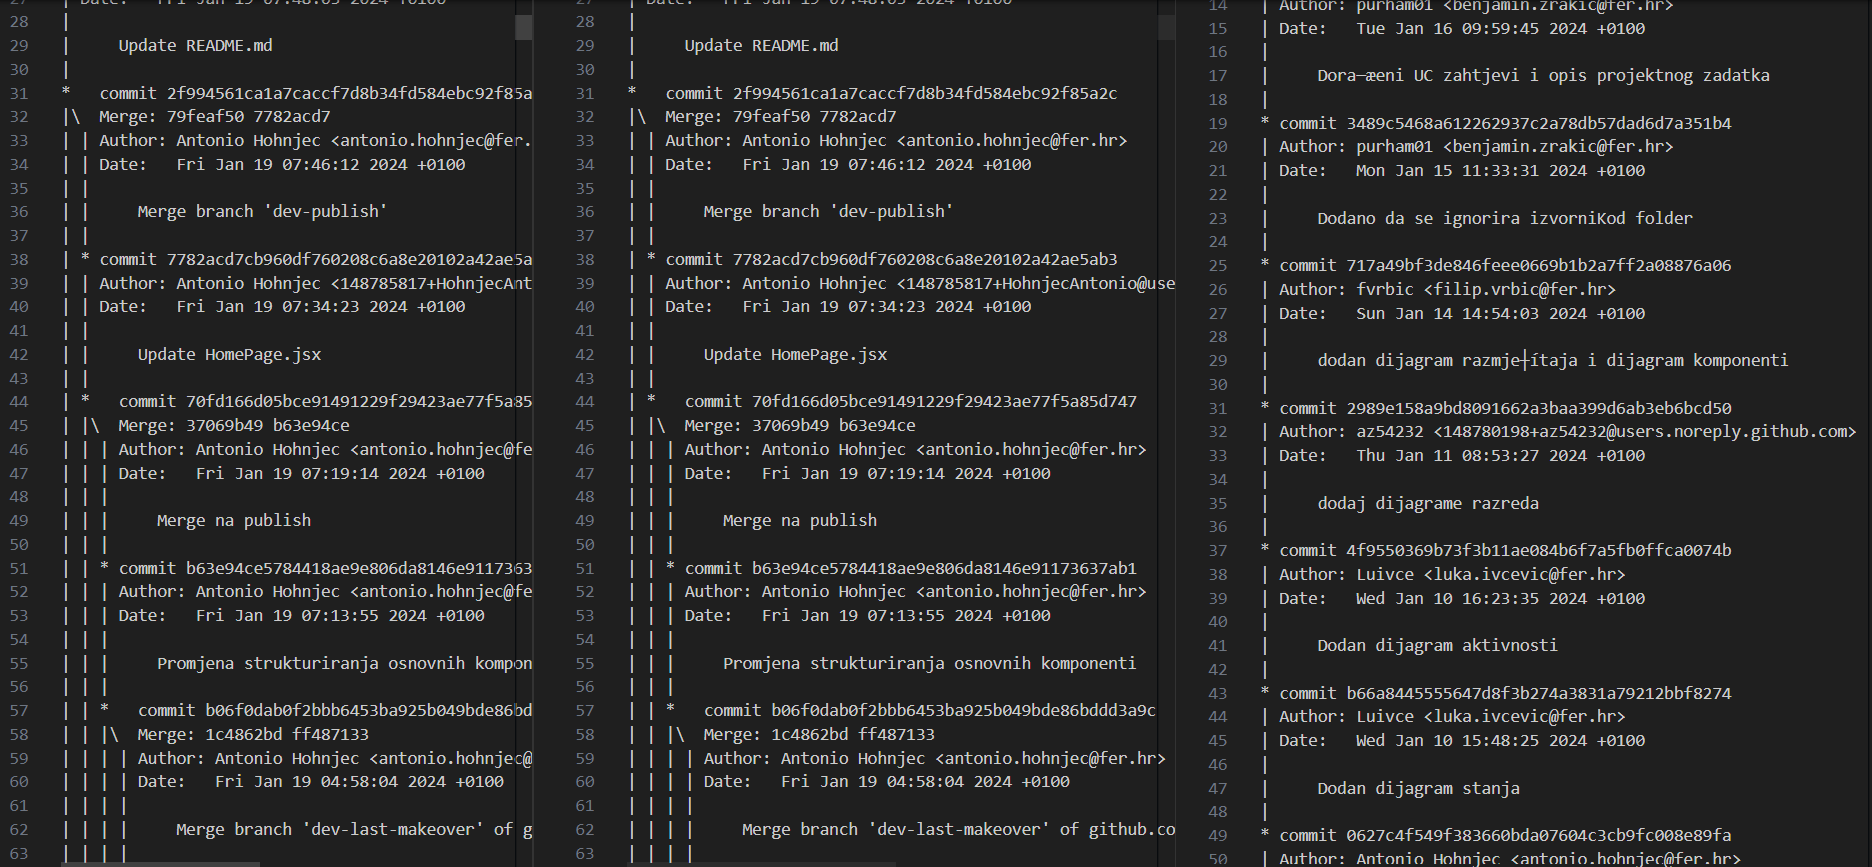
\includegraphics[scale= 0.45]{slike/Logs.png}
			\centering
			\caption{Github logs master, publish i dokumentacija grana}
			\label{fig:Github logs}
		\end{figure} 
	


\end{document} %naredbe i tekst nakon ove naredbe ne ulaze u izgrađen dokument 


